% !TEX program = xelatex
\documentclass[UTF8,zihao=-4,openany]{ctexrep}

\usepackage[a4paper,left=3.0cm,right=2.5cm,top=2.5cm,bottom=2.5cm,headheight=15pt]{geometry}
\usepackage{fontspec}
\IfFontExistsTF{Times New Roman}{\setmainfont{Times New Roman}}{\setmainfont{TeX Gyre Termes}}
\IfFontExistsTF{Menlo}{\setmonofont{Menlo}[Scale=0.86]}{\setmonofont{Latin Modern Mono}[Scale=0.88]}
\IfFontExistsTF{Songti SC}{\setCJKmainfont{Songti SC}}{\setCJKmainfont{FandolSong-Regular}}
\IfFontExistsTF{Heiti SC}{\setCJKsansfont{Heiti SC}}{\setCJKsansfont{FandolHei-Regular}}
\IfFontExistsTF{PingFang SC}{\setCJKmonofont{PingFang SC}}{\setCJKmonofont{FandolFang-Regular}}

\usepackage{amsmath,amssymb}
\usepackage{graphicx}
\usepackage{float}
\usepackage{booktabs}
\usepackage{longtable}
\usepackage{tabularx}
\usepackage{array}
\usepackage{enumitem}
\usepackage{xcolor}
\usepackage{listings}
\usepackage{seqsplit}
\usepackage{caption}
\usepackage{fancyhdr}
\usepackage{setspace}
\usepackage[hidelinks]{hyperref}

\graphicspath{{figures/}}
\linespread{1.35}
\setlength{\parindent}{2em}
\setlength{\parskip}{0pt}
\setlength{\emergencystretch}{2em}
\setlist{nosep}

\pagestyle{fancy}
\fancyhf{}
\fancyhead[C]{数据库原理2大作业期末报告}
\fancyfoot[C]{\thepage}

\numberwithin{figure}{chapter}
\numberwithin{table}{chapter}
\renewcommand{\thefigure}{\thechapter-\arabic{figure}}
\renewcommand{\thetable}{\thechapter-\arabic{table}}
\captionsetup[figure]{name=图,labelsep=quad,font=small,justification=centering}
\captionsetup[table]{name=表,labelsep=quad,font=small,justification=centering}

\ctexset{
  chapter={name={第,章},number=\arabic{chapter},format=\centering\heiti\zihao{3},beforeskip=12pt,afterskip=24pt},
  section={format=\heiti\zihao{4},beforeskip=12pt,afterskip=8pt},
  subsection={format=\heiti\zihao{-4},beforeskip=10pt,afterskip=6pt}
}

\lstdefinestyle{sqlstyle}{
  language=SQL,
  basicstyle=\ttfamily\small,
  keywordstyle=\bfseries\color{blue!60!black},
  commentstyle=\itshape\color{gray!70!black},
  stringstyle=\color{red!50!black},
  breaklines=true,
  columns=fullflexible,
  keepspaces=true,
  frame=single,
  numbers=left,
  numberstyle=\tiny,
  xleftmargin=2em,
  framexleftmargin=1.5em,
  tabsize=4,
  showstringspaces=false
}
\lstdefinestyle{codestyle}{
  basicstyle=\ttfamily\small,
  breaklines=true,
  columns=fullflexible,
  keepspaces=true,
  frame=single,
  numbers=left,
  numberstyle=\tiny,
  xleftmargin=2em,
  framexleftmargin=1.5em,
  tabsize=4,
  showstringspaces=false
}

\newcommand{\systemname}{学生选课成绩管理系统}
\newcommand{\coursename}{数据库原理2}
\newcommand{\reporttitle}{基于 openGauss 的学生选课成绩管理系统数据库设计与实现分析}
\newcommand{\code}[1]{\begingroup\ttfamily\expandafter\seqsplit\expandafter{\detokenize{#1}}\endgroup}

\begin{document}

\begin{titlepage}
  \centering
  \vspace*{2.4cm}
  {\zihao{1}\heiti \reporttitle \par}
  \vspace{1.2cm}
  {\zihao{3}\heiti 数据库原理2大作业期末报告 \par}
  \vspace{2.2cm}
  \begin{table}[H]
    \centering
    \zihao{4}
    \renewcommand{\arraystretch}{1.6}
    \begin{tabular}{rl}
      课程名称： & \coursename \\
      项目名称： & \systemname \\
      数据库平台： & openGauss \\
      应用技术： & Python、Streamlit、psycopg2、Docker \\
      学生姓名： & 请填写姓名 \\
      学号： & 请填写学号 \\
      专业班级： & 请填写专业班级 \\
      完成日期： & \today \\
    \end{tabular}
  \end{table}
  \vfill
  {\zihao{-4} 本报告依据当前项目仓库真实 SQL、服务层代码和运行脚本撰写 \par}
\end{titlepage}

\chapter*{摘要}
\addcontentsline{toc}{chapter}{摘要}

本文以一个面向高校教务场景的\systemname 为研究对象，按照数据库系统生命周期和数据库设计流程，完成从规划、需求分析、概念结构设计、逻辑结构设计、规范化设计、完整性约束、事务并发控制、物理设计到运行维护的数据库设计报告。项目当前使用 Docker 运行 openGauss，应用层采用 Python、Streamlit 和 psycopg2，通过原生 SQL 访问数据库。

报告重点不是介绍页面功能，而是围绕数据库原理课程内容分析系统的数据模型。系统在数据库原理1已有选课系统功能基础上，进一步从数据库原理2的角度优化数据结构和完整性机制：使用 ER 图和关系模型完成概念设计、逻辑设计，将课程定义与教学班分离，使用 \code{enrollment} 将学生与教学班之间的多对多联系转换为关系模式；通过 \code{course_schedule} 将上课时间片结构化，将已选人数和绩点等可计算信息放在视图或规则表查询中获得，避免在基础表中保存复合文本或派生数据；通过主键、外键、唯一约束、CHECK 约束、视图和触发器维护实体完整性、参照完整性和用户自定义完整性。当前数据库层已经实现角色档案一致性、先修课程合法性、选课完整性、教室容量一致性和成绩变更审计触发器；在选课流程中使用 \code{select_course_tx()}、\code{DBSession} 和 \code{SELECT ... FOR UPDATE} 锁定目标教学班，以降低并发抢课导致超选的风险；并通过 \code{test_triggers_constraints.sql} 和 \code{test_grade_policy.sql} 对关键规则进行回滚型验证。系统通过视图统计已选人数，通过 \code{grade_policy} 和 \code{grade_scale} 支持绩点规则版本化，没有在基础表中保存 \code{selected_count} 或 \code{gpa_point} 派生字段。

通过该项目可以较完整地体现数据库设计流程、ER 建模、关系模型转换、范式分析、完整性约束、事务 ACID、锁机制、索引设计和运行维护等数据库原理2课程知识点。

\noindent\textbf{关键词：} openGauss；选课系统；ER 模型；关系模型；3NF；完整性约束；事务；行级锁

\clearpage
\tableofcontents
\clearpage

\chapter{绪论与系统规划}

\section{项目背景}

本项目是一个面向高校教务场景的学生选课成绩管理系统。系统需要支撑学生查询课程、提交选课和退课申请，教师录入成绩并查看成绩分布，管理员维护学期、课程、教学班、学生和教师基础资料。与普通信息展示系统相比，选课系统的核心难点在于数据联系复杂、完整性约束多、并发选课场景明显。课程容量、重复选课、上课时间冲突、先修课程、成绩录入和退课限制都属于典型数据库规则。

项目当前采用 Python + Streamlit 实现界面，使用 psycopg2 连接 openGauss 数据库。数据库部署相关文件位于 \code{opengauss_setup/docker/}，核心建表脚本位于 \code{opengauss_setup/sql/init.sql}。项目没有使用 ORM，也没有使用 Alembic 等迁移框架，数据库模式主要由 SQL 文件维护。

\section{系统规划目标}

根据数据库设计流程，规划阶段首先需要明确系统边界和数据管理目标。本系统的规划目标包括：

\begin{enumerate}
  \item 建立统一的用户账号与角色体系，支持学生、教师、管理员三类用户。
  \item 区分课程定义和具体教学班，支持同一课程在不同学期、不同教师、不同教室开设。
  \item 使用选课记录表达学生和教学班之间的多对多联系，并保存选课状态、选课时间和最终成绩。
  \item 通过结构化上课时间支持时间冲突检查。
  \item 通过主键、外键、唯一约束、CHECK 约束和服务层校验共同保证数据完整性。
  \item 在并发选课场景中使用事务和锁机制降低超选风险。
\end{enumerate}

\section{数据库设计流程说明}

本报告按照数据库设计流程组织章节：需求分析识别角色、功能、数据和规则；概念设计使用 ER 模型抽象实体和联系；逻辑设计把 ER 模型转换为关系模式；规范化设计分析函数依赖和范式；完整性设计讨论主键、外键、CHECK、UNIQUE 和应用层校验；事务与锁章节分析并发选课一致性；物理设计讨论数据类型、索引和性能；运行维护章节说明初始化、部署、安全和扩展。

\section{本章课程知识点}

本章对应数据库系统设计流程中的规划阶段。规划阶段强调数据库系统建设的必要性、系统边界、软硬件环境、数据范围和设计目标。本项目的数据中心特征明显：无论学生选课、教师录入成绩还是管理员维护教学班，本质上都是围绕数据库中实体、联系和约束展开的操作。

\chapter{需求分析}

\section{用户角色}

项目通过 \code{user_account.role} 区分 \code{admin}、\code{student}、\code{teacher} 三类角色。登录认证由 \code{services/auth_service.py} 实现，页面访问控制由 \code{pages/_guards.py} 中的 \code{require_role()} 完成。三类用户需求如下：

\begin{itemize}
  \item 学生：查看当前学期可选课程，提交选课，查看已选课程，按规则退课，查看成绩单和绩点。
  \item 教师：查看本人负责的开课班次，录入或修改学生成绩，查看成绩分布和成绩修改日志。
  \item 管理员：维护学期、课程、开课班次、学生、教师，查看系统统计和所有班次成绩。
\end{itemize}

\section{功能需求}

系统功能需求和真实代码对应关系见表 \ref{tab:function-requirements}。

{\footnotesize
\setlength{\tabcolsep}{3pt}
\renewcommand{\arraystretch}{1.16}
\begin{longtable}{p{2.7cm}p{6.7cm}p{3.9cm}}
\caption{功能需求与项目文件对应关系}\label{tab:function-requirements}\\
\toprule
功能 & 当前实现 & 主要文件 \\
\midrule
\endfirsthead
\toprule
功能 & 当前实现 & 主要文件 \\
\midrule
\endhead
登录与会话 & 用户名密码登录，Cookie 持久会话，按角色进入不同页面 & \code{services/auth_service.py}、\code{utils/auth_cookie.py}、\code{opengauss_setup/sql/add_user_session.sql} \\
课程查询 & 学生、教师、管理员均可通过服务层查询课程与开课班次 & \code{services/course_service.py} \\
选课 & 检查重复、容量、学期状态、选课窗口、先修课、时间冲突后写入 \code{enrollment} & \code{services/selection_service.py} \\
退课 & 只能退本人已选且未录入成绩的课程，并检查学期和时间窗口 & \code{services/selection_service.py} \\
课程与教学班管理 & 管理员维护课程、学期、开课班次和上课时间片 & \code{services/course_service.py}、\code{pages/course_manage.py} \\
成绩管理 & 教师只能维护本人班次，管理员可维护全部班次，并记录成绩日志 & \code{services/score_service.py}、\code{pages/score_manage.py} \\
基础资料维护 & 管理学生、教师资料并同步创建账号 & \code{services/student_service.py}、\code{services/teacher_service.py} \\
\bottomrule
\end{longtable}
}

\section{数据需求}

系统需要保存的数据分为五类。第一类是组织结构数据，包括 \code{department}、\code{major}、\code{classroom}。第二类是用户身份数据，包括 \code{user_account}、\code{user_session}、\code{student}、\code{teacher}、\code{admin_profile}。第三类是教学安排数据，包括 \code{semester}、\code{course}、\code{course_offering}、\code{course_schedule} 和 \code{course_prerequisite}。第四类是选课成绩数据，即 \code{enrollment}。第五类是审计数据，即 \code{score_change_log}。

\section{业务规则}

当前已经实现的业务规则包括：

\begin{enumerate}
  \item 重复选课限制：\code{select_course_tx()} 会锁定并检查同一学生、同一教学班的已有选课记录，\code{enrollment} 表上的 \code{UNIQUE(student_id, offering_id)} 作为数据库层兜底。
  \item 容量限制：\code{trg_enrollment_guard} 在锁定 \code{course_offering} 行后统计 \code{status='selected'} 的人数，并与 \code{max_capacity} 比较。
  \item 行级锁保护：选课函数和选课触发器均使用 \code{SELECT ... FOR UPDATE} 锁定目标 \code{course_offering} 行。
  \item 时间冲突检查：\code{trg_enrollment_guard} 通过 \code{course_schedule} 的 \code{weekday}、\code{start_section}、\code{end_section} 判断同学期区间重叠。
  \item 先修课限制：\code{trg_enrollment_guard} 通过 \code{course_prerequisite} 和历史 \code{completed} 成绩判断先修课是否达到 60 分。
  \item 退课规则：只能退本人 \code{selected} 状态且未录入成绩的记录；数据库触发器禁止已完成或已有成绩的记录退课。
  \item 成绩权限：教师只能维护自己负责的班次，管理员可以维护所有班次。
  \item 成绩范围：数据库 CHECK 与服务层均限制成绩为 0 到 100。
  \item 成绩审计：\code{trg_score_change_log} 在 \code{final_score} 变化后自动写入 \code{score_change_log}，操作者由成绩更新事务传入。
  \item 角色档案一致性：学生、教师、管理员档案由触发器检查其 \code{user_id} 对应账户角色是否匹配。
  \item 教学班与教室容量一致性：\code{trg_offering_capacity_check} 和 \code{trg_classroom_capacity_update_check} 维护 \code{max_capacity} 与教室容量之间的跨表约束。
\end{enumerate}

仍需进一步完善的规则包括：同一学生同一学期选择同一课程不同教学班的限制、数据库级角色授权、备份恢复流程以及多连接并发压测。

\section{数据字典草案}

\begin{longtable}{p{3.4cm}p{3.8cm}p{7cm}}
\caption{核心数据字典草案}\label{tab:data-dictionary}\\
\toprule
数据项 & 来源表 & 含义 \\
\midrule
\endfirsthead
\toprule
数据项 & 来源表 & 含义 \\
\midrule
\endhead
\code{student_id} & \code{student} & 学生业务编号，学生主键。 \\
\code{teacher_id} & \code{teacher} & 教师业务编号，教师主键。 \\
\code{course_id} & \code{course} & 课程编号，表示课程定义。 \\
\code{offering_id} & \code{course_offering} & 教学班代理主键，表示某学期某教师开设的具体课次。 \\
\code{schedule_id} & \code{course_schedule} & 上课时间片主键。 \\
\code{enrollment_id} & \code{enrollment} & 选课记录主键。 \\
\code{final_score} & \code{enrollment} & 学生在某教学班的最终成绩。 \\
\code{token_hash} & \code{user_session} & 持久登录 token 的哈希值。 \\
\bottomrule
\end{longtable}

\chapter{概念结构设计}

\section{实体抽取}

根据当前 \code{init.sql} 反向抽取，系统实体可以分为组织结构、用户身份、教学安排、选课成绩和审计记录五组。

\begin{itemize}
  \item 组织结构实体：院系 \code{department}、专业 \code{major}、教室 \code{classroom}。
  \item 用户身份实体：统一账号 \code{user_account}、学生 \code{student}、教师 \code{teacher}、管理员资料 \code{admin_profile}、用户会话 \code{user_session}。
  \item 教学安排实体：学期 \code{semester}、课程 \code{course}、开课班次 \code{course_offering}、上课时间片 \code{course_schedule}、先修关系 \code{course_prerequisite}。
  \item 选课成绩实体：选课记录 \code{enrollment}。
  \item 审计实体：成绩修改日志 \code{score_change_log}。
\end{itemize}

\section{属性设计}

课程和开课班次是本项目概念设计的关键。课程 \code{course} 保存课程号、课程名、课程类型、学分、学时、所属院系和状态；开课班次 \code{course_offering} 保存课程、学期、教师、教室、容量上限和班次状态。二者分离后，同一课程可在不同学期、不同教师、不同教室多次开设，而不会重复保存课程名称、学分、学时等基础信息。

本次 3NF 重构后，旧的自由文本上课时间不再保存在 \code{course_offering} 中，而是由 \code{course_schedule(schedule_id, offering_id, weekday, start_section, end_section)} 表示。一个教学班可对应多个时间片，便于后续进行时间冲突检查。

\section{联系与基数}

主要联系如下：

\begin{itemize}
  \item 院系与专业、教师、课程均为 1:N。
  \item 统一账号与学生、教师、管理员资料为 1:0..1。
  \item 课程与开课班次为 1:N。
  \item 学期与开课班次为 1:N。
  \item 教师与开课班次为 1:N。
  \item 教室与开课班次为 1:N。
  \item 开课班次与上课时间片为 1:N。
  \item 学生与开课班次是 M:N，通过 \code{enrollment} 转换为两个 1:N 联系。
  \item 课程与课程之间存在先修自关联，通过 \code{course_prerequisite} 转换。
\end{itemize}

\section{ER 图}

\begin{figure}[htbp]
    \centering
    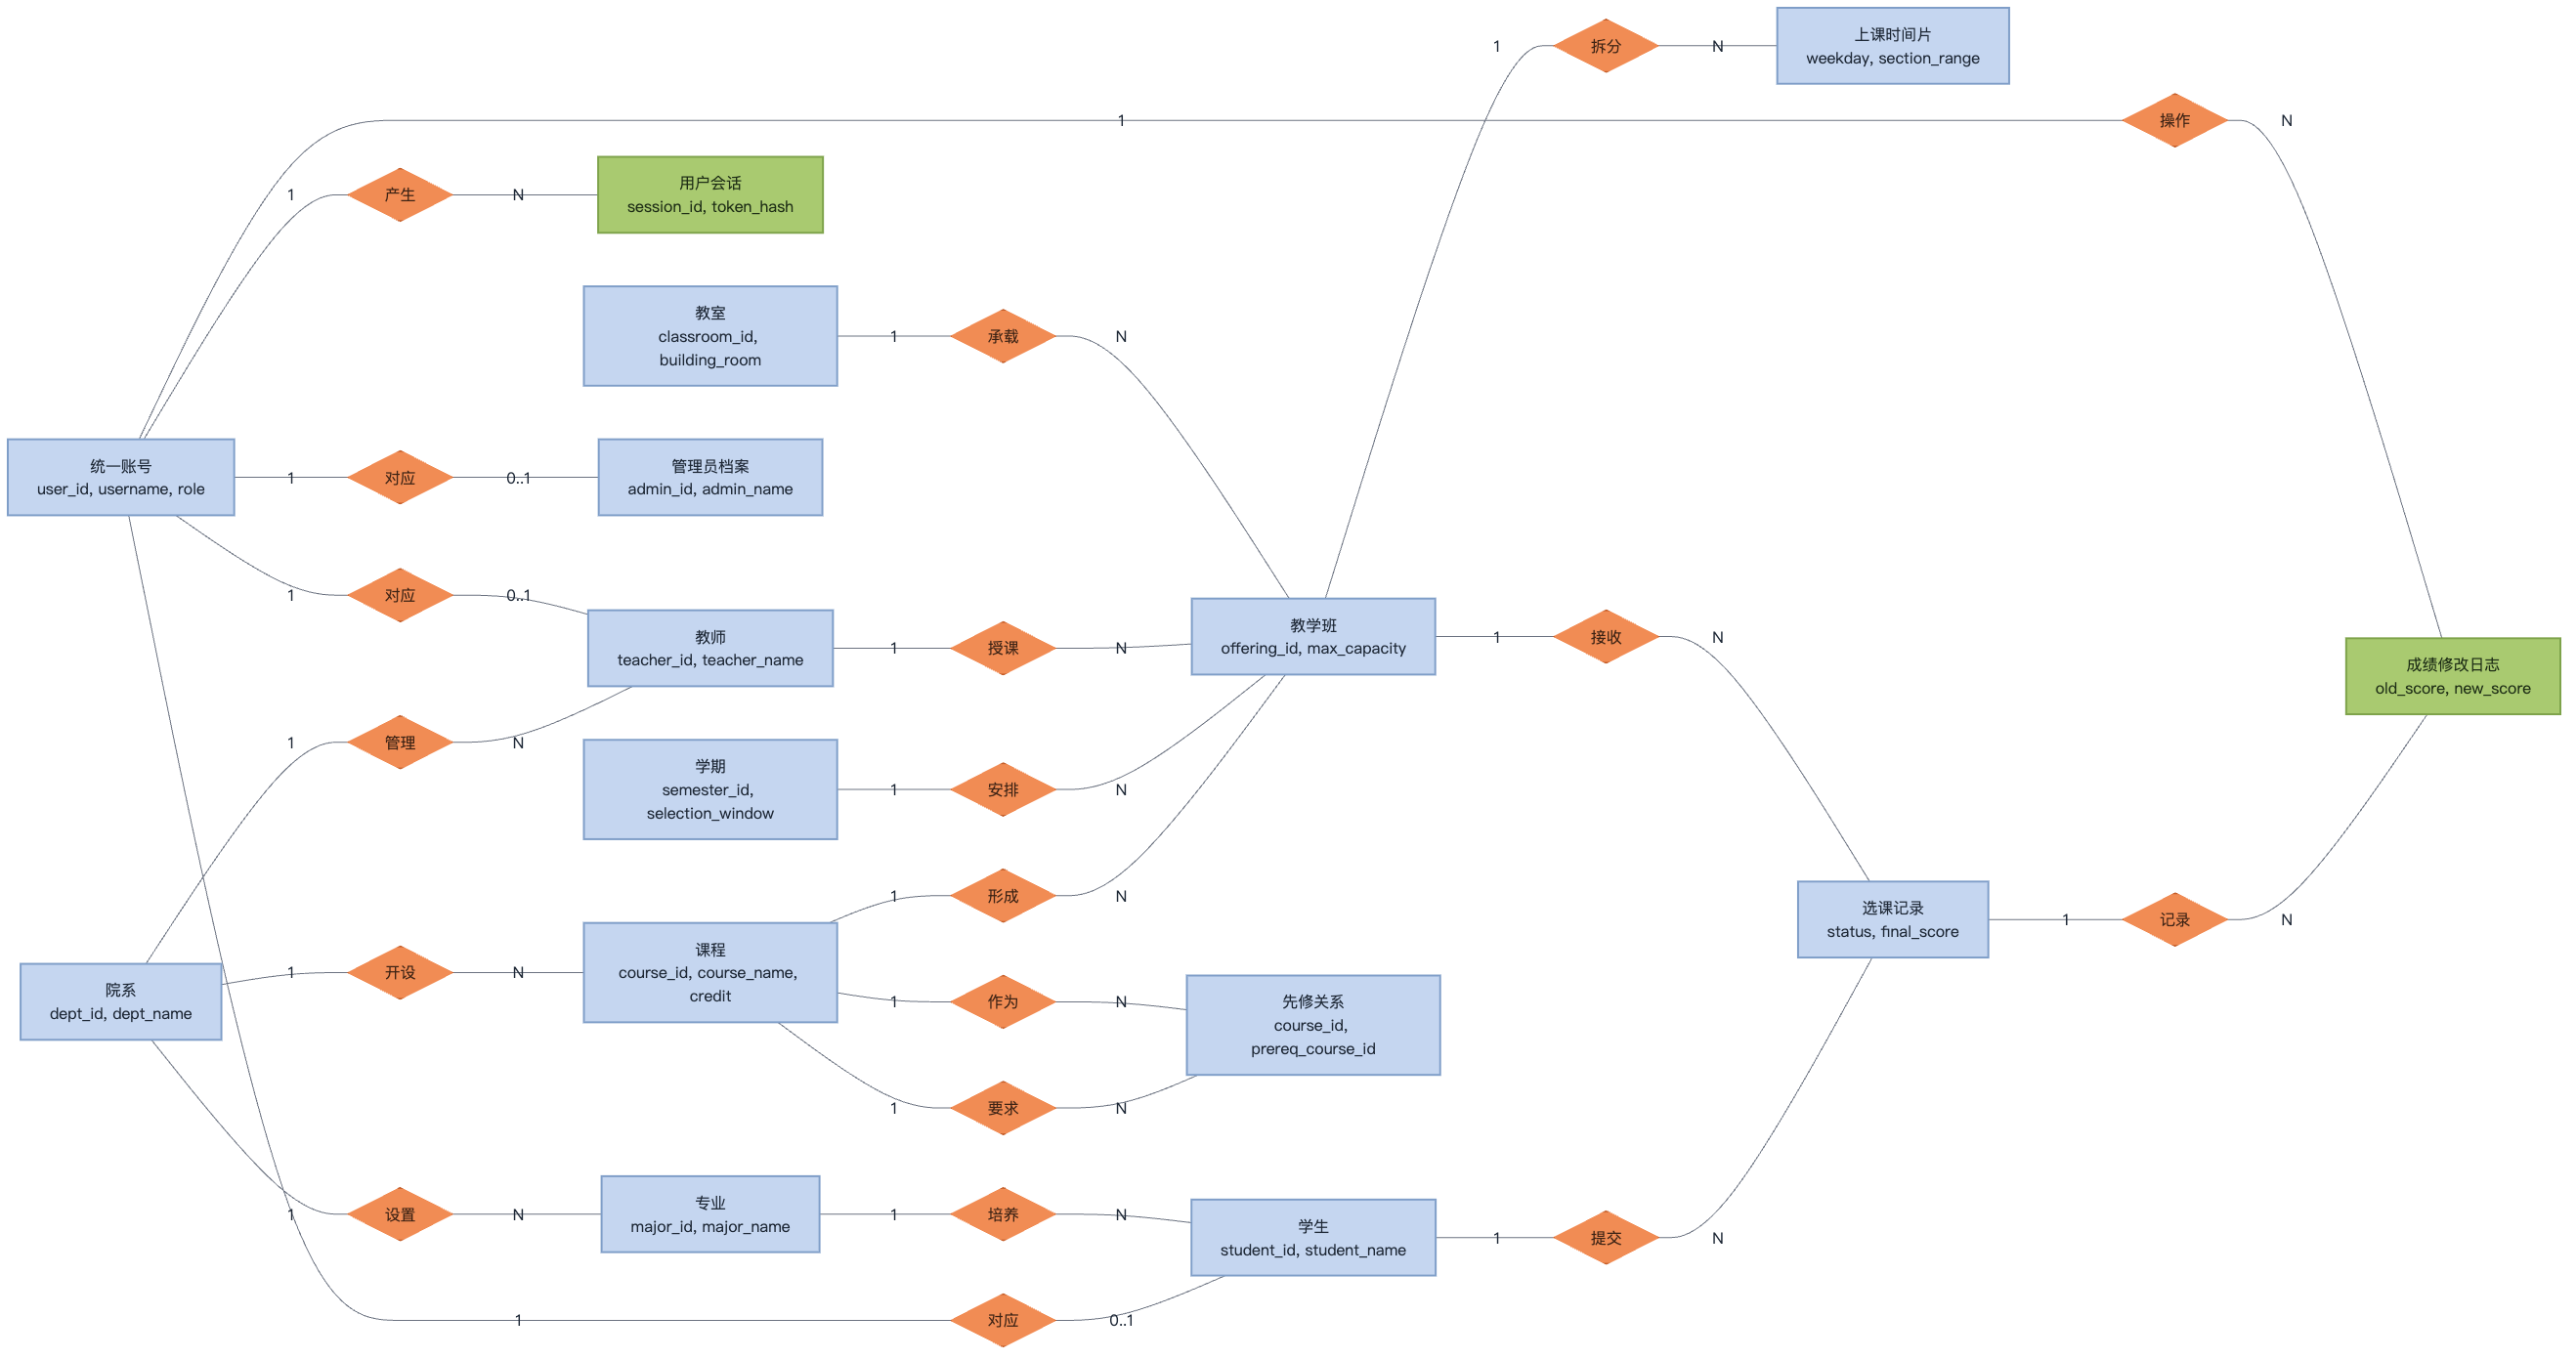
\includegraphics[width=0.98\textwidth]{er_conceptual.png}
    \caption{选课系统概念结构 ER 图}
    \label{fig:er-conceptual}
\end{figure}

图 \ref{fig:er-conceptual} 展示了系统核心实体和联系。图中字段名后缀 \code{_pk}、\code{_fk}、\code{_uk} 分别表示主键、外键和唯一约束。由于 Mermaid ER 图语法限制，复合约束以字段名后缀方式标注。

\section{从业务语义到概念模型}

学生并不是直接选择“课程定义”，而是选择某个学期中由某位教师开设的具体教学班。因此，将学生与课程直接建模为 M:N 会丢失教师、学期、教室、容量和时间等重要语义。本项目使用 \code{course_offering} 表示教学班，再用 \code{enrollment} 表示学生选择教学班这一联系，既符合现实业务，也便于记录选课状态和成绩。

先修关系是课程与课程之间的自关联。如果直接在 \code{course} 中保存一个先修课程字段，只能表达一个先修课程且不利于扩展。当前使用 \code{course_prerequisite(course_id, prereq_course_id)}，可以表达一门课程有多个先修课，也可以表达一门课被多门后续课依赖。

\chapter{逻辑结构设计}

\section{关系模式}

由概念模型转换得到的主要关系模式如下。表名和字段均依据 \code{opengauss_setup/sql/init.sql}。

\begin{itemize}
  \item \code{Department(dept_id, dept_name, office_phone, office_location)}
  \item \code{Major(major_id, major_name, dept_id)}
  \item \code{UserAccount(user_id, username, password_hash, role, status, last_login_at, created_at)}
  \item \code{UserSession(session_id, user_id, token_hash, created_at, expires_at, revoked_at, last_seen_at)}
  \item \code{Student(student_id, user_id, student_name, gender, birth_date, enroll_year, major_id, class_name, phone, email, status)}
  \item \code{Teacher(teacher_id, user_id, teacher_name, gender, dept_id, title, phone, email, status)}
  \item \code{AdminProfile(admin_id, user_id, admin_name, phone)}
  \item \code{Semester(semester_id, semester_name, start_date, end_date, selection_start, selection_end, status)}
  \item \code{Course(course_id, course_name, course_type, credit, total_hours, dept_id, description, status)}
  \item \code{Classroom(classroom_id, building, room_no, capacity)}
  \item \code{CourseOffering(offering_id, course_id, semester_id, teacher_id, classroom_id, max_capacity, status)}
  \item \code{CourseSchedule(schedule_id, offering_id, weekday, start_section, end_section)}
  \item \code{CoursePrerequisite(course_id, prereq_course_id)}
  \item \code{Enrollment(enrollment_id, student_id, offering_id, select_time, status, final_score, remark)}
  \item \code{ScoreChangeLog(log_id, enrollment_id, old_score, new_score, changed_by_user_id, changed_at, reason)}
\end{itemize}

\section{关系模式、主键、外键与唯一约束}

\code{init.sql} 为所有核心表设置主键，并通过外键维护主要参照完整性。表 \ref{tab:logical-schema-constraints} 汇总了当前主要关系模式的键约束。

{\footnotesize
\setlength{\tabcolsep}{3pt}
\renewcommand{\arraystretch}{1.18}
\begin{longtable}{p{0.17\textwidth}p{0.17\textwidth}p{0.37\textwidth}p{0.20\textwidth}}
\caption{关系模式、主键、外键与唯一约束}\label{tab:logical-schema-constraints}\\
\toprule
关系模式 & 主键 & 主要外键 & 唯一约束 / 候选键 \\
\midrule
\endfirsthead
\toprule
关系模式 & 主键 & 主要外键 & 唯一约束 / 候选键 \\
\midrule
\endhead
\bottomrule
\endfoot

\code{department} & \code{dept_id} & 无 & \code{UNIQUE(dept_name)} \\
\code{major} & \code{major_id} & \code{dept_id -> department.dept_id} & \code{UNIQUE(dept_id, major_name)} \\
\code{user_account} & \code{user_id} & 无 & \code{UNIQUE(username)} \\
\code{user_session} & \code{session_id} & \code{user_id -> user_account.user_id} & \code{UNIQUE(token_hash)} \\
\code{student} & \code{student_id} & \code{user_id -> user_account.user_id}；\code{major_id -> major.major_id} & \code{UNIQUE(user_id)} \\
\code{teacher} & \code{teacher_id} & \code{user_id -> user_account.user_id}；\code{dept_id -> department.dept_id} & \code{UNIQUE(user_id)} \\
\code{admin_profile} & \code{admin_id} & \code{user_id -> user_account.user_id} & \code{UNIQUE(user_id)} \\
\code{semester} & \code{semester_id} & 无 & 无显式业务唯一约束 \\
\code{course} & \code{course_id} & \code{dept_id -> department.dept_id} & 无显式业务唯一约束 \\
\code{classroom} & \code{classroom_id} & 无 & \code{UNIQUE(building, room_no)} \\
\code{course_offering} & \code{offering_id} & \code{course_id -> course.course_id}；\code{semester_id -> semester.semester_id}；\code{teacher_id -> teacher.teacher_id}；\code{classroom_id -> classroom.classroom_id} & 无显式复合业务唯一约束 \\
\code{course_schedule} & \code{schedule_id} & \code{offering_id -> course_offering.offering_id} & \code{UNIQUE(offering_id, weekday, start_section, end_section)} \\
\code{course_prerequisite} & \code{course_id, prereq_course_id} & 两列均引用 \code{course.course_id} & 复合主键即业务候选键 \\
\code{enrollment} & \code{enrollment_id} & \code{student_id -> student.student_id}；\code{offering_id -> course_offering.offering_id} & \code{UNIQUE(student_id, offering_id)} \\
\code{score_change_log} & \code{log_id} & \code{enrollment_id -> enrollment.enrollment_id}；\code{changed_by_user_id -> user_account.user_id} & 无显式业务唯一约束 \\

\end{longtable}
}

\section{多对多关系转换}

学生与开课班次之间是 M:N。若直接把课程列表保存在学生表中，会产生列表型字段并破坏 1NF；若把学生列表保存在开课班次表中，同样不利于查询和约束。当前设计使用 \code{enrollment} 作为中间表，把 M:N 转换为：

\begin{itemize}
  \item \code{student} 与 \code{enrollment} 的 1:N；
  \item \code{course_offering} 与 \code{enrollment} 的 1:N。
\end{itemize}

同时，\code{enrollment} 自身具有 \code{select_time}、\code{status}、\code{final_score} 和 \code{remark} 等联系属性，因此它不只是简单连接表，也是描述选课过程和成绩结果的业务实体。\code{UNIQUE(student_id, offering_id)} 防止同一学生重复选择同一教学班。

\section{课程定义与开课班次分离}

当前系统已经正确分离 \code{course} 与 \code{course_offering}。\code{course} 保存稳定的课程定义，例如课程名称、课程类型、学分、总学时和所属学院；\code{course_offering} 保存某课程在某学期由某教师、某教室开设的具体教学班次。若二者不分离，则同一课程每次开班都要重复保存课程名、学分、学时等信息，课程定义调整时容易产生更新异常。

\code{semester}、\code{teacher} 和 \code{classroom} 也独立成表，使 \code{course_offering} 只保存外键和班次自身属性 \code{max_capacity}、\code{status}。该设计有利于后续支持同一课程多学期、多教师、多教学班开设。

\section{多值属性与自关联关系处理}

\code{course_schedule} 是 \code{course_offering} 多值时间属性的拆分结果。一个教学班可以有多个上课时间片，因此逻辑设计中将“上课时间”从 \code{course_offering} 中拆出为独立关系，每行表示一个 \code{weekday, start_section, end_section} 组合。这种设计避免了在开课表中保存 \code{schedule_text} 这类复合文本字段。

\code{course_prerequisite} 是 \code{course} 对 \code{course} 的自关联关系。它使用 \code{course_id} 和 \code{prereq_course_id} 作为复合主键，分别引用同一张 \code{course} 表，用于表达一门课程可以有多门先修课程、一门课程也可以作为多门课程的先修课程。

\section{逻辑关系模型图}

\begin{figure}[htbp]
    \centering
    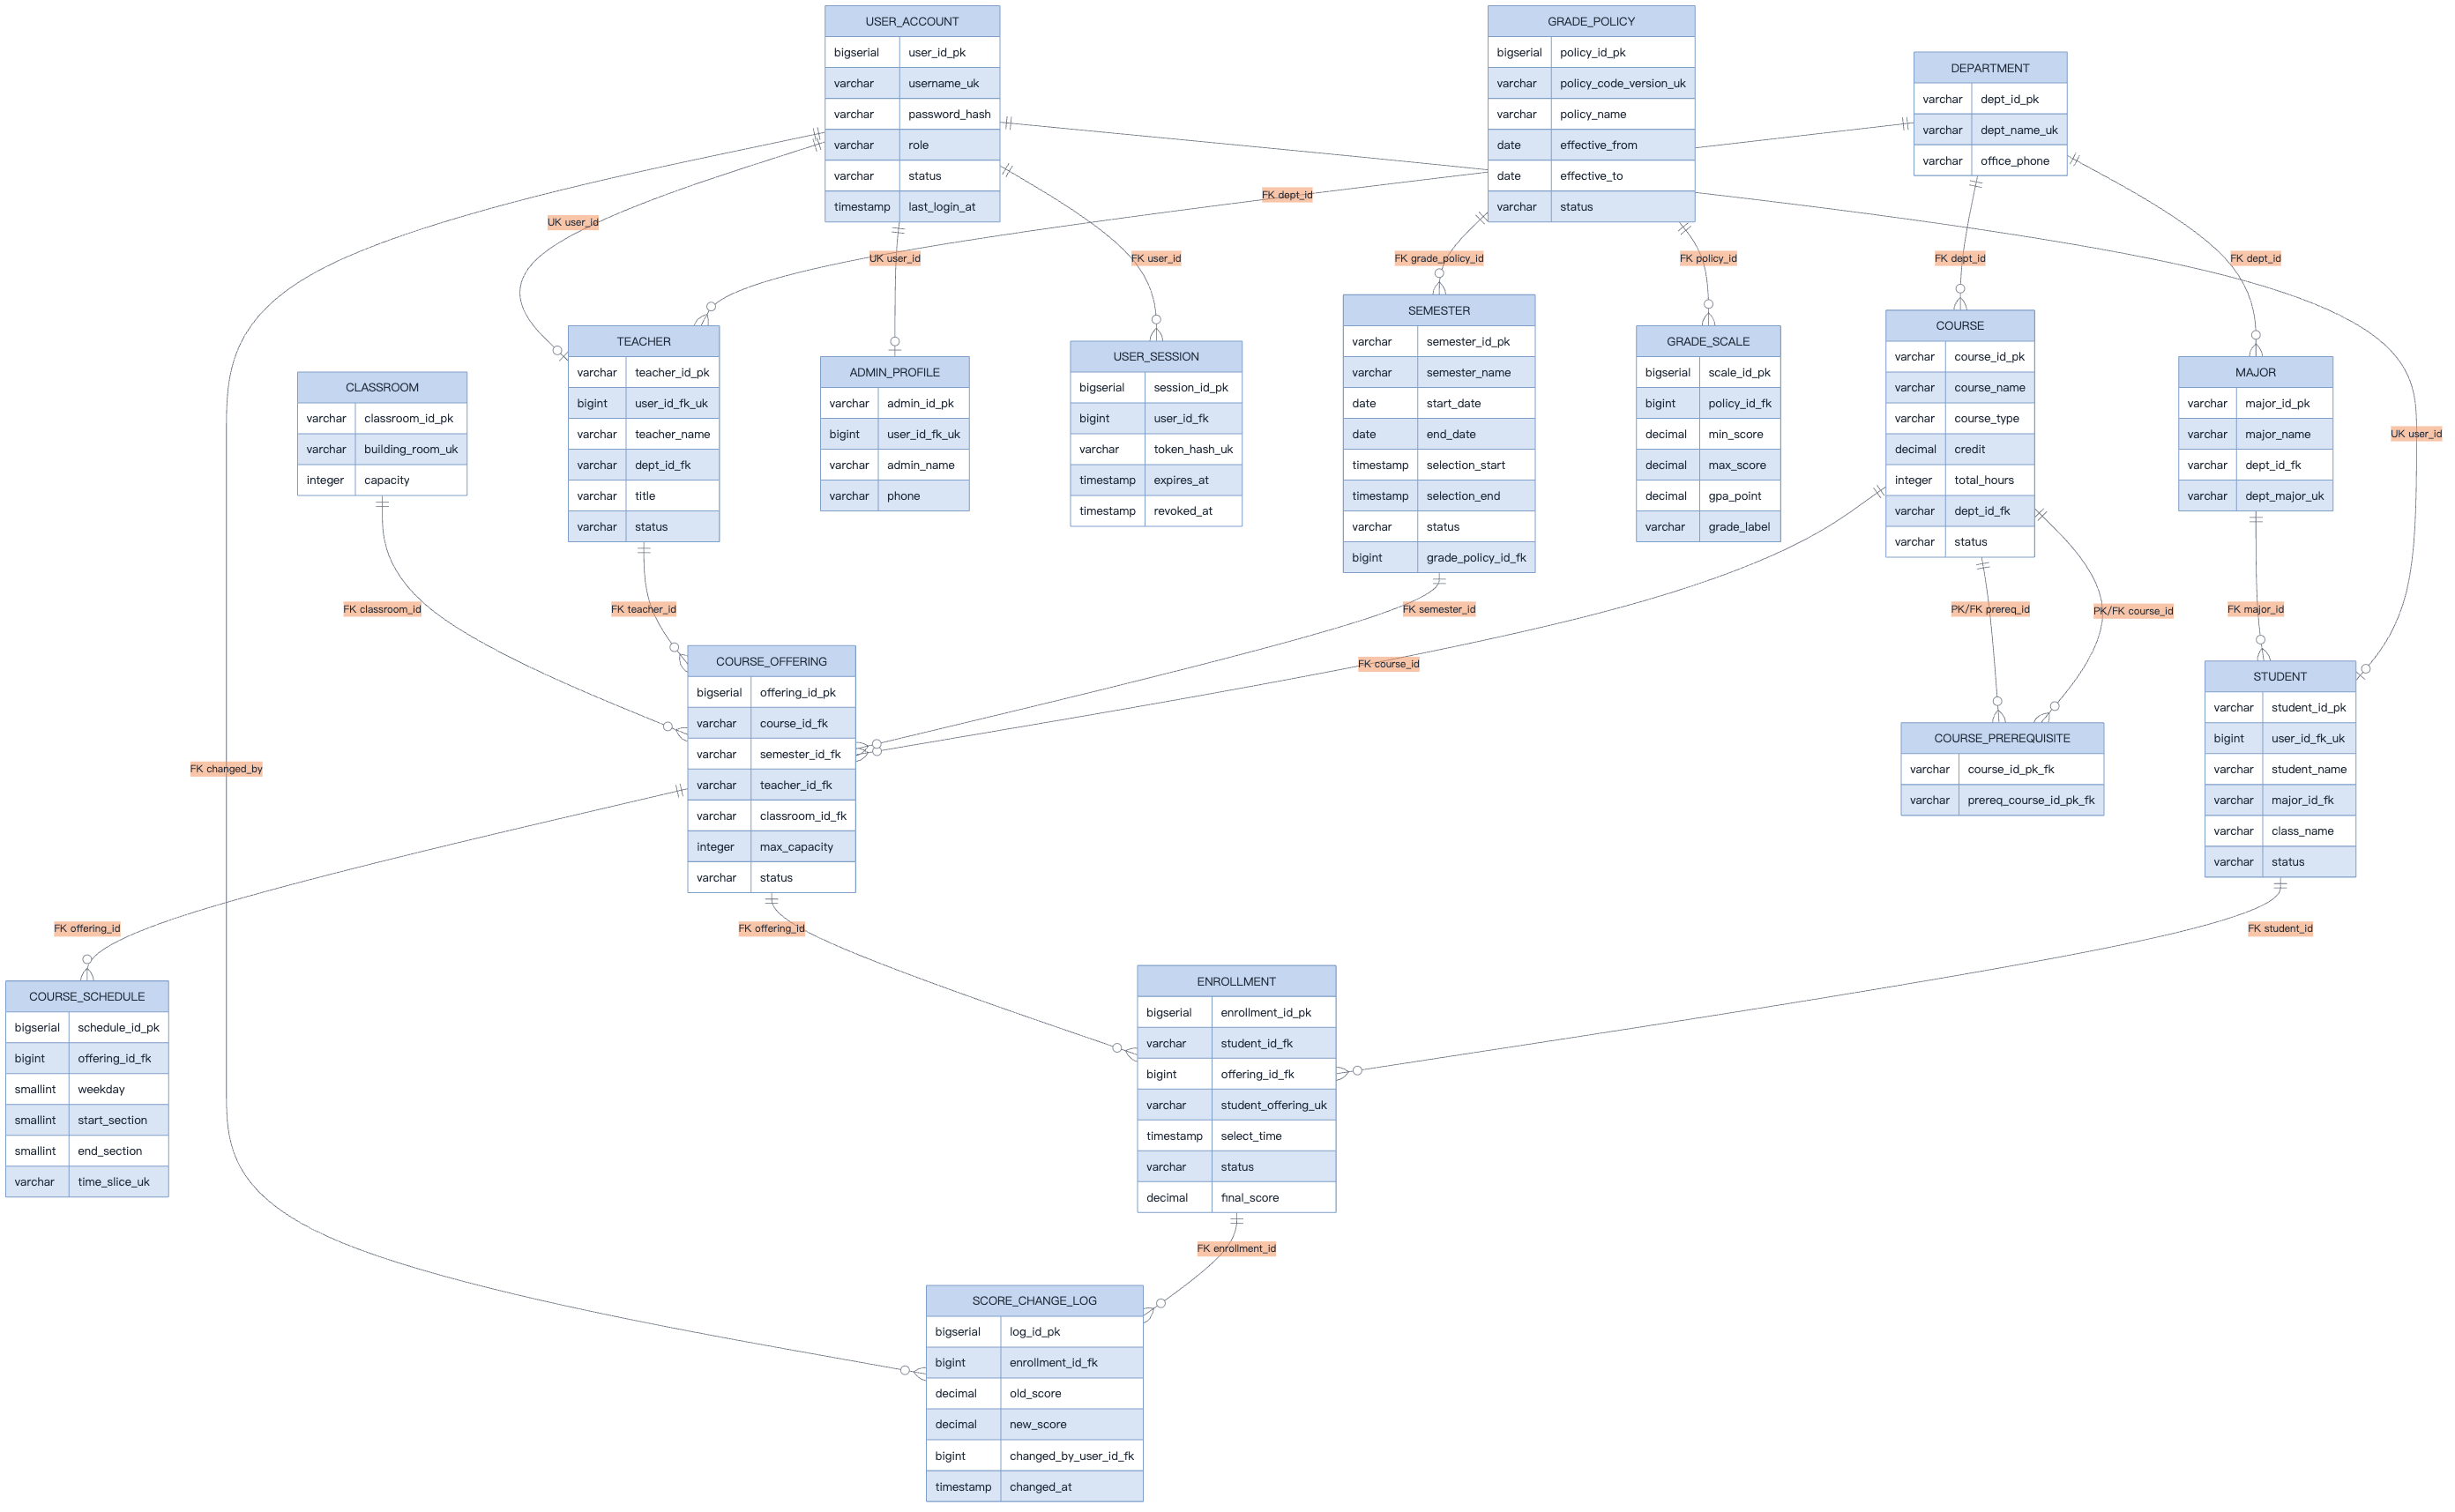
\includegraphics[width=0.98\textwidth]{er_logical.png}
    \caption{选课系统逻辑关系模型图}
    \label{fig:er-logical}
\end{figure}

\section{参照完整性}

当前系统使用外键保证主要参照完整性。例如，选课记录必须引用存在的学生和教学班；开课班次必须引用存在的课程、学期和教师；上课时间片必须引用存在的开课班次；成绩变更日志必须引用存在的选课记录和操作账号。值得注意的是，\code{user_session.user_id} 和 \code{course_schedule.offering_id} 使用 \code{ON DELETE CASCADE}，分别用于在删除账号时清理会话、在删除无选课记录的教学班时清理时间片。

部分跨表业务规则无法仅靠普通外键表达，当前已经通过触发器补充其中的核心规则：\code{course_offering.max_capacity <= classroom.capacity} 由教学班和教室容量触发器维护，账户角色与具体档案表之间的一致性由角色档案触发器维护。仍需改进的是同一学生同一学期不重复选择同一课程的不同教学班，这类规则需要在后续通过跨表触发器、培养方案规则表或更细的业务键设计实现。

\chapter{规范化设计与范式分析}

\section{规范化分析对象与方法}

规范化设计的目标是在保证业务语义完整表达的前提下，减少数据冗余，避免插入异常、删除异常和更新异常。本章不单独停留在范式概念说明，而是以系统当前数据库 schema 为对象，对核心关系模式进行函数依赖、候选键、第一范式、第二范式、第三范式和 BCNF 分析。主要依据为 \code{opengauss_setup/sql/init.sql}、\code{opengauss_setup/sql/migrate_3nf_20260608.sql} 和 \code{opengauss_setup/sql/add_user_session.sql}。

当前系统已经将组织结构、账户认证、角色档案、课程定义、开课班次、上课时间、选课记录和成绩变更日志拆分为相对独立的关系模式。该设计体现了从 ER 模型到关系模型的转换过程，也为完整性约束、事务控制和后续维护提供了基础。需要特别说明的是，本章只把 SQL 中已经存在的表、字段、主键、外键、唯一约束、CHECK 约束、触发器和视图作为“当前实现”；绩点规则表、行政班实体等尚未落地的机制仍作为后续改进讨论。

\section{当前关系模式与主键、候选键、外键}

从业务模块看，当前数据库可以分为四类关系模式。

\begin{enumerate}[label=（\arabic*）]
    \item 组织结构模块：\code{department}、\code{major}；
    \item 账户与角色模块：\code{user_account}、\code{user_session}、\code{student}、\code{teacher}、\code{admin_profile}；
    \item 课程教学模块：\code{semester}、\code{course}、\code{classroom}、\code{course_offering}、\code{course_schedule}、\code{course_prerequisite}；
    \item 选课成绩模块：\code{enrollment}、\code{score_change_log}。
\end{enumerate}

这种划分避免了把登录信息、学生档案、课程定义、具体开课、选课关系和成绩日志混合在单张大表中，从整体上降低了数据冗余和更新异常风险。表 \ref{tab:normalization-audit} 按关系模式列出主键、候选键、主要函数依赖和范式判断。

{\scriptsize
\setlength{\tabcolsep}{2pt}
\renewcommand{\arraystretch}{1.18}
\begin{longtable}{p{0.13\textwidth}p{0.17\textwidth}p{0.27\textwidth}p{0.16\textwidth}p{0.19\textwidth}}
\caption{核心关系模式的函数依赖与范式审计}\label{tab:normalization-audit}\\
\toprule
关系模式 & 主键 / 候选键 & 主要函数依赖 & 范式判断 & 说明 \\
\midrule
\endfirsthead
\toprule
关系模式 & 主键 / 候选键 & 主要函数依赖 & 范式判断 & 说明 \\
\midrule
\endhead
\bottomrule
\endfoot

\code{department} &
\code{dept_id} &
\code{dept_id} $\rightarrow$ \code{dept_name}, \code{office_phone}, \code{office_location} &
3NF，具有 BCNF 倾向 &
已补充 \code{uq_department_name}，学院名称也成为显式业务唯一决定因素。 \\

\code{major} &
\code{major_id} &
\code{major_id} $\rightarrow$ \code{major_name}, \code{dept_id} &
3NF，具有 BCNF 倾向 &
通过 \code{dept_id} 引用学院，且已补充 \code{uq_major_dept_name} 避免同院系专业重名。 \\

\code{user_account} &
\code{user_id}；\code{username} &
\code{user_id} $\rightarrow$ \code{username}, \code{password_hash}, \code{role}, \code{status}；\code{username} $\rightarrow$ \code{user_id} &
3NF/BCNF 倾向明显 &
\code{username} 有唯一约束，是登录业务候选键。 \\

\code{user_session} &
\code{session_id}；\code{token_hash} &
\code{session_id} $\rightarrow$ \code{user_id}, \code{token_hash}, \code{created_at}, \code{expires_at}, \code{revoked_at}；\code{token_hash} $\rightarrow$ \code{session_id} &
3NF/BCNF 倾向明显 &
会话独立成表，避免在账户表中保存多个 token，符合 1NF。 \\

\code{student} &
\code{student_id}；\code{user_id} &
\code{student_id} $\rightarrow$ \code{user_id}, \code{student_name}, \code{gender}, \code{major_id}, \code{class_name}, \code{status}；\code{user_id} $\rightarrow$ \code{student_id} &
3NF，BCNF 需结合业务语义 &
学生档案与账户分离；\code{major_id} 外键避免保存专业和院系详细信息。 \\

\code{teacher} &
\code{teacher_id}；\code{user_id} &
\code{teacher_id} $\rightarrow$ \code{user_id}, \code{teacher_name}, \code{dept_id}, \code{title}, \code{status}；\code{user_id} $\rightarrow$ \code{teacher_id} &
3NF，BCNF 需结合业务语义 &
教师档案独立，避免账户表膨胀，并通过 \code{dept_id} 引用学院。 \\

\code{admin_profile} &
\code{admin_id}；\code{user_id} &
\code{admin_id} $\rightarrow$ \code{user_id}, \code{admin_name}, \code{phone}；\code{user_id} $\rightarrow$ \code{admin_id} &
3NF/BCNF 倾向明显 &
管理员资料与认证信息分离，\code{user_id} 唯一表达一对一关系。 \\

\code{semester} &
\code{semester_id} &
\code{semester_id} $\rightarrow$ \code{semester_name}, \code{start_date}, \code{end_date}, \code{selection_start}, \code{selection_end}, \code{status} &
3NF，具有 BCNF 倾向 &
学期日期和选课窗口独立保存，避免在开课表中重复。 \\

\code{course} &
\code{course_id} &
\code{course_id} $\rightarrow$ \code{course_name}, \code{course_type}, \code{credit}, \code{total_hours}, \code{dept_id}, \code{status} &
3NF，BCNF 需结合业务语义 &
保存课程定义，不保存具体学期、教师或教室。 \\

\code{classroom} &
\code{classroom_id} &
\code{classroom_id} $\rightarrow$ \code{building}, \code{room_no}, \code{capacity} &
3NF，BCNF 需补充候选键确认 &
教室容量独立保存；已补充 \code{uq_classroom_location} 避免重复教室实体。 \\

\code{course_offering} &
\code{offering_id} &
\code{offering_id} $\rightarrow$ \code{course_id}, \code{semester_id}, \code{teacher_id}, \code{classroom_id}, \code{max_capacity}, \code{status} &
3NF，具有 BCNF 倾向 &
表示某课程在某学期由某教师开设的教学班，不再保存 \code{schedule_text} 和 \code{selected_count}。 \\

\code{course_schedule} &
\code{schedule_id}；\code{offering_id, weekday, start_section, end_section} &
\code{schedule_id} $\rightarrow$ \code{offering_id}, \code{weekday}, \code{start_section}, \code{end_section} &
1NF/2NF/3NF 良好 &
将上课时间拆为结构化时间片，业务唯一约束防止同一班次重复时间片。 \\

\code{course_prerequisite} &
\code{course_id, prereq_course_id} &
无非主属性 &
2NF/3NF/BCNF 倾向明显 &
复合主键表，无非主属性，因此无部分依赖和传递依赖。 \\

\code{enrollment} &
\code{enrollment_id}；\code{student_id, offering_id} &
\code{enrollment_id} $\rightarrow$ \code{student_id}, \code{offering_id}, \code{select_time}, \code{status}, \code{final_score}, \code{remark}；\code{student_id, offering_id} $\rightarrow$ \code{enrollment_id} &
3NF，具有 BCNF 倾向 &
选课关系表，同时保存状态、时间和成绩等联系属性；不再保存 \code{gpa_point}。 \\

\code{score_change_log} &
\code{log_id} &
\code{log_id} $\rightarrow$ \code{enrollment_id}, \code{old_score}, \code{new_score}, \code{changed_by_user_id}, \code{changed_at}, \code{reason} &
3NF，具有 BCNF 倾向 &
成绩修改历史独立保存，并由成绩更新触发器自动写入审计日志。 \\

\end{longtable}
}

\section{核心函数依赖分析}

根据当前 SQL 结构，主要函数依赖可以分为实体标识依赖、业务候选键依赖和联系属性依赖三类。

第一类是实体标识依赖。例如，\code{dept_id} 决定学院名称、办公电话和办公地点；\code{course_id} 决定课程名称、课程类型、学分、学时和所属学院；\code{classroom_id} 决定楼栋、房间号和容量。这类依赖由主键直接表达。

第二类是业务候选键依赖。例如，\code{user_account.username} 有唯一约束，因此 \code{username} 可以决定 \code{user_id} 及账户状态；\code{user_session.token_hash} 有唯一约束，因此 token 摘要可以决定对应会话；\code{student.user_id}、\code{teacher.user_id}、\code{admin_profile.user_id} 均具有唯一约束，用于表达账户与角色档案之间的一对一关系。

第三类是联系属性依赖。典型代表是 \code{enrollment}：\code{student_id, offering_id} 共同决定一条选课记录，\code{select_time}、\code{status}、\code{final_score}、\code{remark} 都依赖于“一名学生选择一个教学班”这一完整联系，而不是只依赖学生或只依赖教学班。

本次 3NF 迁移重点删除了若干派生依赖风险：\code{course_offering.selected_count} 可由 \code{enrollment} 聚合得到；\code{enrollment.gpa_point} 可由 \code{final_score} 和绩点规则推导；\code{course_offering.schedule_text} 则把多个时间片压入一个文本字段。这些字段不再保存在基础表中。

\section{第一范式分析：属性原子性与结构化时间片}

第一范式要求关系中的每个属性都是不可再分的原子值，不能在一个字段中保存列表、集合或重复组。当前系统最典型的 1NF 改造体现在上课时间设计中。

旧设计如果将上课时间保存为 \code{course_offering.schedule_text}，例如“周一 1-2 节 / 周三 3-4 节”，则一个字段中同时包含多个时间片。该设计虽然便于页面展示，但不利于数据库按星期和节次进行查询，也不利于选课时间冲突检查。当前设计将其拆分为 \code{course_schedule} 表，每条记录只表示一个教学班的一个上课时间片，包括 \code{weekday}、\code{start_section} 和 \code{end_section}。这样，每个字段都具有清晰的原子语义，满足第一范式要求。

\code{migrate_3nf_20260608.sql} 也体现了这一改造路径：脚本先创建 \code{course_schedule}，再使用 \code{REGEXP_SPLIT_TO_TABLE} 将旧的 \code{schedule_text} 按分隔符解析为多行结构化时间片，最后删除 \code{course_offering.schedule_text}。迁移脚本同时提醒，如果历史数据中存在自定义格式的上课时间文本，需要在删除旧字段前人工检查解析结果。

此外，\code{user_session} 表没有在 \code{user_account} 中保存多个登录 token，而是将每次会话独立成行；\code{course_prerequisite} 没有在 \code{course} 中使用字符串列表保存先修课程，而是使用自关联中间表表达课程之间的先修关系。这些设计都避免了多值字段，提高了结构化查询能力。

\section{第二范式分析：复合键与部分函数依赖}

第二范式要求在满足第一范式的基础上，非主属性必须完全函数依赖于候选键，而不能只依赖复合键的一部分。对于使用单属性代理主键的关系模式，部分函数依赖问题通常不明显；本系统中更需要重点分析的是具有复合业务键的关系。

\code{course_prerequisite} 的主键为 \code{course_id, prereq_course_id}，表中没有额外非主属性，因此不存在非主属性只依赖 \code{course_id} 或只依赖 \code{prereq_course_id} 的问题。该表的意义是把课程对课程的先修多对多关系转换为关系模式。

\code{course_schedule} 虽然使用 \code{schedule_id} 作为代理主键，但其业务唯一约束为 \code{offering_id, weekday, start_section, end_section}。该组合共同决定一个具体时间片，表中没有诸如课程名称、教师姓名、教室容量等只依赖 \code{offering_id} 的冗余字段，因此不存在明显部分依赖。

\code{enrollment} 使用 \code{enrollment_id} 作为代理主键，同时使用 \code{student_id, offering_id} 作为业务候选键。选课时间、选课状态、最终成绩和备注都描述一次具体选课关系，而不是只描述学生或只描述教学班。因此这些属性依赖完整的选课关系，满足第二范式要求。

\section{第三范式分析：传递依赖、派生字段与表分解}

第三范式要求在满足第二范式的基础上，非主属性之间不应存在传递函数依赖。当前系统通过多处表分解减少了传递依赖。

在组织结构设计中，\code{student} 表只保存 \code{major_id}，不直接保存学院名称、学院电话或学院办公地点；\code{major} 表保存 \code{dept_id}；\code{department} 表保存学院详细信息。这样避免了在学生表中出现 \code{student_id} $\rightarrow$ \code{major_id} $\rightarrow$ \code{dept_name} 的传递依赖。类似地，\code{teacher} 和 \code{course} 也只通过 \code{dept_id} 引用学院，而不重复保存学院详细信息。

在课程设计中，\code{course} 保存课程定义，\code{course_offering} 保存具体开课班次，\code{semester}、\code{teacher}、\code{classroom} 分别保存学期、教师和教室信息。开课班次表只保存这些实体的外键，而不重复保存课程名称、教师姓名、学期起止日期或教室容量，从而减少了更新异常。

账户设计也体现了表分解思想。\code{user_account} 保存登录账号、密码哈希、角色、状态和最近登录时间；\code{student}、\code{teacher}、\code{admin_profile} 分别保存不同角色的业务档案，并通过唯一的 \code{user_id} 与账户建立一对一关系。这种设计避免了把学生、教师和管理员的差异化字段堆在同一张账户表中。本轮已经通过 \code{trg_student_role_check}、\code{trg_teacher_role_check} 和 \code{trg_admin_role_check} 强制档案表引用的账户角色与档案类型一致。

第三范式改造中最重要的部分是删除派生字段。旧设计中的 \code{course_offering.selected_count} 可以通过 \code{enrollment} 表按教学班和选课状态统计得到。如果同时在开课表中保存已选人数，则每次选课、退课或状态变更都必须同步更新该字段，一旦事务失败或并发控制不当，就可能出现容量统计不一致。当前 3NF 迁移删除该字段，体现了消除派生冗余的设计思路。服务层需要显示已选人数时，通过 \code{COUNT(*)} 或子查询动态计算；如果未来数据量很大，可以考虑视图、物化视图或受控冗余，而不是简单恢复 \code{selected_count}。

类似地，旧设计中的 \code{enrollment.gpa_point} 可以由 \code{final_score} 和绩点换算规则推导。如果直接存储绩点，当成绩被修改时，绩点也必须同步修改，否则会产生更新异常。因此迁移脚本删除 \code{gpa_point}。当前 \code{services/score_service.py} 和 \code{services/course_service.py} 在查询时用 CASE 表达式生成展示用绩点。如果后续系统确实需要管理不同年份、不同课程或不同学院的绩点换算规则，应设计 \code{grade_policy} 或 \code{grade_scale} 表保存规则，再通过查询或视图计算绩点。

\code{score_change_log} 的存在不属于上述派生字段冗余。它保存的是成绩修改事件历史，包含旧成绩、新成绩、修改人、修改时间和原因。若只在 \code{enrollment} 中覆盖 \code{final_score}，历史成绩会丢失；独立日志表反而增强了审计能力。本轮已经实现 \code{trg_score_change_log}，成绩变更由数据库触发器自动写入日志。

\section{BCNF 分析：决定因素与候选键}

BCNF 要求每一个非平凡函数依赖的决定因素都必须是候选键。与 3NF 相比，BCNF 对决定因素要求更严格，因此不能在证据不足时简单宣称所有关系模式都完全满足 BCNF。

在当前 SQL 已声明的主键、唯一约束和主要业务语义下，多数核心关系模式的决定因素是主键或候选键，因此具有较好的 BCNF 倾向。比如，\code{user_account} 中 \code{user_id} 和 \code{username} 都可以作为候选键；\code{student}、\code{teacher}、\code{admin_profile} 中 \code{user_id} 也通过唯一约束表达与账户的一对一关系；\code{enrollment} 中 \code{student_id, offering_id} 作为业务候选键防止重复选课；\code{course_schedule} 中 \code{offering_id, weekday, start_section, end_section} 表示唯一时间片。

但 BCNF 的严格判断依赖业务语义。本轮已经将 \code{dept_name}、\code{building, room_no}、\code{dept_id, major_name} 这三类业务唯一性显式声明为 UNIQUE 约束，使这些业务决定因素成为候选键。由此，\code{department}、\code{major} 和 \code{classroom} 在当前业务语义下的 BCNF 说明更加充分。

因此，本系统当前设计在主键和已声明唯一约束范围内具有较好的 BCNF 倾向。但如果未来继续增加新的业务语义，例如正式行政班编码、绩点规则版本、跨学期培养方案等，仍需要同步声明新的候选键或拆分新的关系模式。

\section{从旧设计到 3NF 的迁移说明}

\code{migrate_3nf_20260608.sql} 是本报告中体现规范化改造的重要证据。该脚本先删除旧的选课触发器和函数，再创建 \code{course_schedule}，迁移历史上课时间文本，最后删除反范式风险字段，并创建补偿查询性能的索引。表 \ref{tab:old-new-3nf} 对旧字段和当前改造进行对比。

{\footnotesize
\setlength{\tabcolsep}{3pt}
\renewcommand{\arraystretch}{1.18}
\begin{longtable}{p{0.22\textwidth}p{0.29\textwidth}p{0.25\textwidth}p{0.16\textwidth}}
\caption{旧设计字段与 3NF 改造说明}\label{tab:old-new-3nf}\\
\toprule
旧设计 & 存在问题 & 当前改造 & 对应范式意义 \\
\midrule
\endfirsthead
\toprule
旧设计 & 存在问题 & 当前改造 & 对应范式意义 \\
\midrule
\endhead
\bottomrule
\endfoot

\code{course_offering.schedule_text} &
一个文本字段包含多个上课时间片，例如“周一 1-2 节 / 周三 3-4 节”，不便于时间冲突检查，也不符合属性原子化要求。 &
迁移到 \code{course_schedule(offering_id, weekday, start_section, end_section)}，迁移脚本解析旧文本后删除该字段。 &
增强 1NF，支持结构化查询。 \\

\code{course_offering.selected_count} &
已选人数由 \code{enrollment} 统计得到，是派生字段，容易在插入、退课和并发选课时产生更新异常。 &
删除 \code{selected_count}，通过 \code{enrollment} 统计或视图获得已选人数。 &
减少冗余，增强 3NF，一致性更好。 \\

\code{enrollment.gpa_point} &
绩点可由 \code{final_score} 和绩点规则推导，直接保存可能与最终成绩不一致。 &
删除 \code{gpa_point}，后续可通过 \code{grade_policy}、\code{grade_scale} 或视图计算。 &
避免派生数据冗余，减少更新异常。 \\

\code{trg_enrollment_insert} / \code{trg_enrollment_update} &
旧设计可能依赖触发器维护 \code{selected_count}，一旦触发器失败或并发复杂，容易产生一致性问题。 &
迁移脚本删除相关触发器和函数，当前转为消除冗余字段。 &
从“维护冗余字段”转向“消除冗余字段”。 \\

\end{longtable}
}

\section{当前设计中仍可改进的规范化问题}

虽然当前设计已经较好地体现了规范化思想，但仍存在若干可以进一步完善的地方。

首先，\code{class_name} 当前作为文本字段保存在 \code{student} 表中。如果班级只是展示标签，该设计可以接受；但如果班级还具有辅导员、年级、所属专业、班级人数等独立属性，则应新增 \code{class} 表，并在 \code{student} 中保存 \code{class_id}，避免班级信息重复。

其次，本轮新增的 \code{uq_department_name}、\code{uq_major_dept_name} 和 \code{uq_classroom_location} 已经把学院名称、同院系专业名称、楼栋房间号等业务唯一性固化到数据库层。这些约束不仅防止重复数据，也能让业务决定因素显式成为候选键，有助于更严格地讨论 BCNF。

再次，\code{course_prerequisite} 当前可以表达课程先修关系。本轮已经增加 \code{chk_prereq_not_self}，避免课程把自己设置为自己的先修课；同时通过 \code{trg_prerequisite_no_cycle} 使用递归查询检测先修课程环路。

最后，如果后续需要绩点计算，应新增 \code{grade_policy} 或 \code{grade_scale} 表，而不是恢复 \code{enrollment.gpa_point}；如果需要高性能课程容量统计，可以用视图、物化视图或受控冗余，而不是直接恢复 \code{selected_count}。这些方案都需要在性能和一致性之间进行权衡。

\section{本章小结}

本章从函数依赖和候选键出发，对系统核心关系模式进行了规范化审计。当前设计通过组织结构分解、账户与角色档案分离、课程定义与开课班次分离、上课时间片结构化、选课关系独立建模和成绩日志独立保存，较好地避免了多值字段、部分依赖和传递依赖。尤其是 \code{course_schedule} 的引入以及 \code{schedule_text}、\code{selected_count}、\code{gpa_point} 的删除，体现了从实现便利型设计向规范化设计的演进过程。本轮新增的业务唯一约束、触发器和视图没有破坏 3NF：视图只是查询层封装，触发器用于维护跨表完整性。后续系统可以继续通过班级实体、绩点规则表和培养方案规则表来提高数据库设计的严谨性。

\chapter{完整性约束、触发器与检查机制}

\section{完整性约束设计目标}

本章依据 \code{opengauss_setup/sql/init.sql}、\code{migrate_triggers_constraints_20260608.sql} 和 \code{test_triggers_constraints.sql}，说明当前系统已经落地的数据库完整性机制。完整性设计目标包括：实体可唯一标识、外键引用合法、业务取值范围合法、角色档案与账户角色一致、先修课程关系无自指和环路、选课过程不超容量且不发生时间冲突、成绩修改可以审计追踪。

与旧版本通过触发器维护 \code{selected_count} 的思路不同，当前系统在 3NF 迁移后删除了 \code{selected_count} 派生字段。本系统不再通过触发器同步该字段，而是通过 \code{enrollment} 表和视图统计当前已选人数。触发器的职责转向跨表业务完整性检查和审计记录维护，例如选课容量检查、时间冲突检查、先修课程合法性检查以及成绩变更日志写入。

\section{实体完整性：主键约束}

实体完整性主要通过主键实现。当前 \code{init.sql} 为所有核心表设置主键，例如 \code{department.dept_id}、\code{student.student_id}、\code{teacher.teacher_id}、\code{course.course_id}、\code{course_offering.offering_id}、\code{course_schedule.schedule_id}、\code{enrollment.enrollment_id}。这些主键保证每个实体或业务事件可以被唯一标识。

\section{参照完整性：外键约束}

参照完整性通过外键约束实现。典型外键包括：\code{major.dept_id} 引用 \code{department.dept_id}，\code{student.user_id} 引用 \code{user_account.user_id}，\code{course_offering.course_id} 引用 \code{course.course_id}，\code{course_schedule.offering_id} 引用 \code{course_offering.offering_id}，\code{enrollment.student_id} 引用 \code{student.student_id}，\code{score_change_log.enrollment_id} 引用 \code{enrollment.enrollment_id}。其中 \code{user_session.user_id} 和 \code{course_schedule.offering_id} 使用 \code{ON DELETE CASCADE}，用于自动清理会话和教学班时间片。

\section{用户自定义完整性：UNIQUE、CHECK、NOT NULL、DEFAULT}

本轮新增的 \code{migrate_triggers_constraints_20260608.sql} 在原有主键、外键、NOT NULL、DEFAULT 和 CHECK 约束基础上，进一步补充了业务唯一约束和合法性检查。表 \ref{tab:constraints-new} 总结了主要约束。

\begin{longtable}{p{0.23\textwidth}p{0.35\textwidth}p{0.33\textwidth}}
\caption{主要完整性约束}\label{tab:constraints-new}\\
\toprule
表 & 约束 & 业务含义 \\
\midrule
\endfirsthead
\toprule
表 & 约束 & 业务含义 \\
\midrule
\endhead
\bottomrule
\endfoot
\code{department} & \code{uq_department_name} & 学院名称唯一，避免同一学院重复建档。 \\
\code{major} & \code{uq_major_dept_name} & 同一学院内专业名称唯一。 \\
\code{classroom} & \code{uq_classroom_location} & 同一楼栋同一房间号只能对应一个教室实体。 \\
\code{course_prerequisite} & \code{chk_prereq_not_self} & 课程不能把自己作为自己的先修课程。 \\
\code{semester} & \code{chk_semester_date_range} & 学期起止日期、选课窗口起止时间必须合法。 \\
\code{user_session} & \code{chk_user_session_time_range} & 会话过期时间必须晚于创建时间，撤销时间不能早于创建时间。 \\
\code{course_schedule} & \code{chk_schedule_section_range} & 节次范围限定为 1 到 12，并要求结束节次不早于开始节次。 \\
\code{enrollment} & \code{UNIQUE(student_id, offering_id)} & 防止同一学生重复选择同一教学班。 \\
\end{longtable}

教学班容量与教室容量的关系属于跨表约束，普通 CHECK 无法查询另一张表，因此本系统使用触发器实现。迁移脚本执行前先审计并修正了已有样例数据中 \code{MA101} 班次容量大于 \code{M201} 教室容量的问题。

\section{跨表业务完整性与触发器设计}

本轮已经实现数据库触发器，触发器定义集中在 \code{opengauss_setup/sql/migrate_triggers_constraints_20260608.sql}。这些触发器不是用于维护 \code{selected_count}，而是用于角色档案一致性、先修关系合法性、选课完整性、教室容量一致性和成绩审计。表 \ref{tab:trigger-list} 给出触发器清单。

{\scriptsize
\setlength{\tabcolsep}{2pt}
\renewcommand{\arraystretch}{1.16}
\begin{longtable}{p{0.17\textwidth}p{0.12\textwidth}p{0.16\textwidth}p{0.25\textwidth}p{0.16\textwidth}p{0.08\textwidth}}
\caption{数据库触发器实现清单}\label{tab:trigger-list}\\
\toprule
触发器名称 & 作用表 & 触发时机 & 检查或维护内容 & 对应课程知识点 & 实现状态 \\
\midrule
\endfirsthead
\toprule
触发器名称 & 作用表 & 触发时机 & 检查或维护内容 & 对应课程知识点 & 实现状态 \\
\midrule
\endhead
\bottomrule
\endfoot
\code{trg_student_role_check} & \code{student} & 插入或修改 \code{user_id} 前 & 学生档案必须引用 \code{role='student'} 的账户 & 跨表用户自定义完整性 & 已实现 \\
\code{trg_teacher_role_check} & \code{teacher} & 插入或修改 \code{user_id} 前 & 教师档案必须引用 \code{role='teacher'} 的账户 & 子类型一致性 & 已实现 \\
\code{trg_admin_role_check} & \code{admin_profile} & 插入或修改 \code{user_id} 前 & 管理员档案必须引用 \code{role='admin'} 的账户 & 角色完整性 & 已实现 \\
\code{trg_prerequisite_no_cycle} & \code{course_prerequisite} & 插入或更新前 & 禁止自指先修课，并用递归查询检测环路 & 递归查询与复杂完整性 & 已实现 \\
\code{trg_offering_capacity_check} & \code{course_offering} & 插入或改容量、教室前 & 教学班容量不能超过教室容量，且不能低于当前已选人数 & 跨表约束 & 已实现 \\
\code{trg_classroom_capacity_update_check} & \code{classroom} & 更新 \code{capacity} 前 & 降低教室容量时不能小于已有教学班容量 & 更新约束 & 已实现 \\
\code{trg_enrollment_guard} & \code{enrollment} & 插入或改学生、班次、状态前 & 检查学生状态、班次状态、选课窗口、容量、时间冲突、先修课和退课限制 & 主动规则、事务与锁 & 已实现 \\
\code{trg_score_change_log} & \code{enrollment} & 更新 \code{final_score} 后 & 自动写入 \code{score_change_log}，记录旧成绩、新成绩、操作者和原因 & 审计触发器 & 已实现 \\
\end{longtable}
}

\section{选课完整性触发器}

\code{trg_enrollment_guard} 是选课系统最核心的数据库层完整性保护。对 \code{status='selected'} 的插入或恢复选课，它会锁定目标 \code{course_offering} 行，然后检查当前已选人数是否小于 \code{max_capacity}。已选人数通过 \code{enrollment} 聚合统计得到，系统没有恢复 \code{course_offering.selected_count}。

该触发器还基于 \code{course_schedule} 检查同一学期内的时间冲突，区间重叠条件为：

\begin{lstlisting}[style=sqlstyle]
target.weekday = existing.weekday
AND existing.start_section <= target.end_section
AND existing.end_section >= target.start_section
\end{lstlisting}

先修课程检查基于 \code{course_prerequisite} 和历史 \code{enrollment} 记录。系统采用 60 分作为通过先修课程的业务规则，即学生必须存在 \code{status='completed'} 且 \code{final_score >= 60} 的先修课程记录。退课时，触发器禁止已完成课程或已有成绩记录改为 \code{dropped}。

\section{成绩变更审计触发器}

\code{trg_score_change_log} 在 \code{enrollment.final_score} 更新后触发。当旧成绩和新成绩不同，触发器自动向 \code{score_change_log} 插入日志。由于日志表要求 \code{changed_by_user_id} 非空，业务层必须在同一事务内设置当前操作者：

\begin{lstlisting}[style=sqlstyle]
SELECT set_config('app.current_user_id', '<user_id>', true);
SELECT set_config('app.score_change_reason', '<reason>', true);
UPDATE enrollment
SET final_score = 88, status = 'completed'
WHERE enrollment_id = 1;
\end{lstlisting}

如果业务层没有设置 \code{app.current_user_id}，触发器会拒绝成绩更新。这比单纯在应用层手工插入日志更可靠，因为任何直接更新 \code{final_score} 的数据库操作都会被同一个审计规则约束。

\section{角色档案一致性触发器}

\code{student}、\code{teacher} 和 \code{admin_profile} 虽然都通过 \code{user_id} 外键引用 \code{user_account}，但普通外键只能保证账户存在，不能保证角色匹配。因此本系统实现了通用函数 \code{check_user_role_fn(p_user_id, p_expected_role)}，并由三个档案触发器复用。测试脚本已经验证，将教师账户插入学生档案、将学生账户插入教师档案都会被拒绝。

\section{先修课程合法性触发器}

\code{chk_prereq_not_self} 可以阻止 \code{course_id = prereq_course_id} 的直接自指，但不能发现更复杂的 A 依赖 B、B 依赖 C、C 又依赖 A 的环路。本系统通过 \code{trg_prerequisite_no_cycle} 在插入或更新先修关系前执行递归查询，沿着先修链查找是否会回到当前课程。如果形成环路，触发器抛出异常并阻止写入。

\section{应用层校验与数据库触发器的关系}

当前应用层仍保留友好的错误提示和页面交互检查，例如 \code{services/selection_service.py} 会调用数据库函数 \code{select_course_tx()}，\code{services/score_service.py} 会在事务内设置审计上下文。数据库触发器承担兜底一致性责任：即使绕过前端或服务层，只要直接写数据库，也必须通过容量、时间冲突、先修课程、角色档案和成绩审计规则。

这种分层体现了数据库完整性设计思想：局部、稳定的规则用 CHECK、UNIQUE 和外键表达；跨表和上下文相关规则用触发器表达；用户体验相关的提示和权限入口仍由应用层负责。

\section{本章小结}

本章说明了当前系统已经从“约束设计方案”推进到“数据库层实现”。主键、外键、唯一约束、CHECK、DEFAULT 保证基础完整性；角色、容量、先修、选课和成绩日志等跨表规则由触发器维护；应用层负责权限入口、事务调用和友好错误提示。尤其需要强调的是，触发器没有恢复 \code{selected_count}，而是在保留 3NF 结构的前提下承担复杂完整性检查和审计职责。

\chapter{事务管理、锁机制与并发控制}

\section{选课系统中的并发一致性问题}

选课系统最典型的并发问题是多个学生同时抢同一教学班的最后一个名额。如果容量检查和写入选课记录不在同一事务隔离边界内，两个事务可能同时读到相同的剩余容量，并分别插入选课记录，最终造成超选。

另一个并发问题是同一学生在多个浏览器窗口重复提交选课请求。该问题一方面由数据库函数和触发器检查已有记录，另一方面由 \code{enrollment} 表上的 \code{UNIQUE(student_id, offering_id)} 在数据库层兜底。

\section{选课事务边界设计}

\code{DBSession} 是项目的事务封装。它进入环境时建立连接，正常退出时提交事务，发生异常时回滚事务。学生选课、退课和成绩更新均使用显式事务路径。

学生选课由选课服务调用数据库函数 \code{select_course_tx(p_student_id, p_offering_id)}。openGauss 存储函数本身不显式开始或提交事务，而是在调用方事务中执行带锁检查和写入。因此事务边界由 \code{DBSession} 管理，数据库函数和触发器在同一事务环境内工作。

\section{选课事务流程}

选课事务流程见表 \ref{tab:select-transaction-flow}。其核心原则是：容量检查、时间冲突检查、先修课程检查和写入 \code{enrollment} 必须处于同一事务边界内。

{\footnotesize
\setlength{\tabcolsep}{3pt}
\renewcommand{\arraystretch}{1.18}
\begin{longtable}{p{0.09\textwidth}p{0.25\textwidth}p{0.17\textwidth}p{0.24\textwidth}p{0.17\textwidth}}
\caption{选课事务流程}\label{tab:select-transaction-flow}\\
\toprule
步骤 & 数据库操作 & 涉及表 & 一致性目标 & 并发控制机制 \\
\midrule
\endfirsthead
\toprule
步骤 & 数据库操作 & 涉及表 & 一致性目标 & 并发控制机制 \\
\midrule
\endhead
\bottomrule
\endfoot
1 & 服务层打开 \code{DBSession} 并调用 \code{select_course_tx()} & 无 & 建立提交或回滚边界 & 应用层事务封装 \\
2 & 查询并锁定同一学生同一教学班的已有记录 & \code{enrollment} & 处理重复选课、退课后恢复或已完成课程重选 & \code{FOR UPDATE} \\
3 & 锁定目标教学班 & \code{course_offering} & 串行化同一班次容量检查 & \code{FOR UPDATE} \\
4 & 插入或更新选课记录 & \code{enrollment} & 形成新的选课关系 & 触发器随语句执行 \\
5 & 检查学生、班次和学期状态 & \code{student}、\code{course_offering}、\code{semester} & 阻止非在读学生或关闭班次选课 & 触发器兜底 \\
6 & 统计当前已选人数 & \code{enrollment} & 防止超过 \code{max_capacity} & 行锁后聚合统计 \\
7 & 检查同课跨班 & \code{course_offering}、\code{enrollment} & 同一学期同一课程只能选择一个教学班 & 同一事务内查询 \\
8 & 检查时间冲突 & \code{course_schedule}、\code{enrollment} & 同一学生同学期课程时间不重叠 & 同一事务内查询 \\
9 & 检查先修课程 & \code{course_prerequisite}、\code{enrollment} & 未通过先修课不能选后续课 & 同一事务内查询 \\
10 & 由唯一约束兜底 & \code{enrollment} & 防止重复记录落库 & \code{UNIQUE(student_id, offering_id)} \\
\end{longtable}
}

关键函数调用形式如下：

\begin{lstlisting}[style=sqlstyle]
SELECT select_course_tx(:student_id, :offering_id);
\end{lstlisting}

该设计把业务检查尽量下沉到数据库层，应用层主要负责开启事务和把数据库异常转换为用户可理解的提示。

\section{行级锁防止并发超选}

防止超选的关键是对目标 \code{course_offering} 行加行级锁。数据库函数和 \code{trg_enrollment_guard} 都使用 \code{SELECT ... FOR UPDATE} 锁定目标教学班：

\begin{lstlisting}[style=sqlstyle]
SELECT course_id, semester_id, max_capacity, status
FROM course_offering
WHERE offering_id = :offering_id
FOR UPDATE;
\end{lstlisting}

当多个事务同时选择同一个教学班时，后到事务必须等待先到事务提交或回滚。已选人数统计发生在获得该行锁之后：

\begin{lstlisting}[style=sqlstyle]
SELECT COUNT(*)
FROM enrollment
WHERE offering_id = :offering_id
  AND status = 'selected';
\end{lstlisting}

由于同一教学班的容量检查被串行化，两个事务不会同时基于同一个未同步的容量视图插入记录，因此可以防止“最后一个名额被多人同时抢到”的超选问题。系统不在基础表中维护 \code{selected_count} 字段，而是通过锁加聚合统计实现一致性。

\section{唯一约束与重复选课防护}

\code{select_course_tx()} 会先查询并锁定同一学生、同一教学班的已有 \code{enrollment} 记录。如果记录已经是 \code{selected}，函数直接拒绝；如果记录已经 \code{completed}，也拒绝重复选择；如果是 \code{dropped}，则尝试恢复为 \code{selected}，并由触发器重新执行容量、时间冲突和先修课程检查。

即使应用层或函数逻辑遗漏，\code{UNIQUE(student_id, offering_id)} 仍会在数据库层拒绝重复记录。这是用唯一约束维护业务候选键的典型做法。

进一步地，\code{trg_enrollment_guard} 已经补充同课跨班限制：同一学生在同一学期如果已经选择某门课程的一个教学班，则不能再选择同一 \code{semester_id}、同一 \code{course_id} 下的另一个教学班。该规则无法仅靠 \code{UNIQUE(student_id, offering_id)} 表达，因为它需要跨 \code{enrollment} 和 \code{course_offering} 查询课程与学期，因此适合由触发器实现。

\section{时间冲突与先修课程检查的事务一致性}

时间冲突和先修课程检查也放在 \code{trg_enrollment_guard} 中执行。由于触发器与触发它的 INSERT 或 UPDATE 语句处在同一事务内，如果检查失败，选课写入会一起回滚。时间冲突使用 \code{course_schedule} 的结构化时间片判断区间重叠；先修课程使用 \code{course_prerequisite} 和历史 \code{completed} 选课记录判断是否达到 60 分。

\section{成绩更新事务与审计一致性}

成绩更新同样采用事务化路径。服务层在同一 \code{DBSession} 中锁定目标 \code{enrollment} 行，检查教师或管理员权限，然后设置审计变量：

\begin{lstlisting}[style=sqlstyle]
SELECT set_config('app.current_user_id', :user_id, true);
SELECT set_config('app.score_change_reason', :reason, true);
UPDATE enrollment
SET final_score = :score, status = 'completed'
WHERE enrollment_id = :enrollment_id;
\end{lstlisting}

\code{trg_score_change_log} 在 \code{final_score} 更新后自动写入 \code{score_change_log}。如果成绩更新失败，日志不会产生；如果日志写入失败，成绩更新也会回滚。因此成绩和审计日志处于同一事务一致性边界内。

\section{事务隔离级别分析}

触发器不是独立事务，而是在触发它的 INSERT 或 UPDATE 语句所在事务中执行。也就是说，\code{trg_enrollment_guard} 抛出异常会使选课语句失败并回滚，\code{trg_score_change_log} 插入日志失败也会使成绩更新失败。这一机制体现了事务的原子性和一致性。

在本系统中，触发器负责数据库层兜底，服务层负责事务入口、用户权限和友好错误提示。二者配合后，选课容量、时间冲突、先修课程、退课限制和成绩日志不再只是前端或服务层约定，而成为数据库可以强制执行的规则。

系统没有显式调整全局事务隔离级别，而是针对高风险资源使用行级锁。对选课容量而言，锁定 \code{course_offering} 行能够把同一教学班的容量检查串行化；对重复选课而言，业务唯一约束可以在较低隔离级别下兜底；对成绩更新而言，服务层锁定目标 \code{enrollment} 行后再更新成绩，避免同一成绩记录并发覆盖。

% \section{多连接并发测试}

% 除回滚型 SQL 测试外，多连接并发验证程序用于模拟两个独立数据库连接同时抢一个容量为 1 的教学班。验证程序创建测试学期、测试课程、两个测试学生和一个容量为 1 的教学班，然后使用两个线程分别调用 \code{select_course_tx()}。并发验证记录结果为 \code{success_count = 1}、\code{failed_count = 1}、\code{selected_count_in_db = 1}。

% 该脚本的价值在于验证 \code{SELECT ... FOR UPDATE} 不只是理论设计，而能在真实多连接环境中串行化同一教学班的容量检查。测试结果表明，在两个事务几乎同时提交选课请求时，只有一个事务成功插入 \code{selected} 记录，另一个事务在锁释放后重新统计容量并因名额已满失败。

% \section{并发控制的不足与改进}

% 表 \ref{tab:concurrency-risk-solution} 汇总了系统面向典型并发场景的处理方式。

% {\footnotesize
% \setlength{\tabcolsep}{3pt}
% \renewcommand{\arraystretch}{1.18}
% \begin{longtable}{p{0.22\textwidth}p{0.23\textwidth}p{0.27\textwidth}p{0.20\textwidth}}
% \caption{并发风险与解决机制}\label{tab:concurrency-risk-solution}\\
% \toprule
% 并发风险 & 可能后果 & 数据库层解决机制 & 应用层配合 \\
% \midrule
% \endfirsthead
% \toprule
% 并发风险 & 可能后果 & 数据库层解决机制 & 应用层配合 \\
% \midrule
% \endhead
% \bottomrule
% \endfoot
% 多个学生同时抢最后一个名额 & 超过 \code{max_capacity} & 锁定 \code{course_offering} 行后统计 \code{enrollment} & \code{DBSession} 调用 \code{select_course_tx()} \\
% 同一学生多窗口重复提交 & 出现重复选课记录 & \code{select_course_tx()} 锁定既有记录，\code{UNIQUE(student_id, offering_id)} 兜底 & 把数据库异常转换为友好提示 \\
% 教师更新成绩时需要审计 & 成绩变更无追踪或日志与成绩不一致 & \code{trg_score_change_log} 与成绩更新同事务执行 & 同事务设置 \code{app.current_user_id} 和修改原因 \\
% 退课与成绩录入并发 & 已录入成绩的课程被退课 & 退课锁定目标 \code{enrollment}，触发器禁止有成绩或已完成记录退课 & 退课接口使用 \code{DBSession} \\
% 管理员修改教学班容量时学生正在选课 & 容量降低造成已选人数超过上限 & \code{trg_offering_capacity_check} 检查容量不能低于当前已选人数 & 管理页面限制容量输入下限 \\
% \end{longtable}
% }

% 系统已处理最核心的抢课容量风险、重复选课风险和同课跨班风险，但仍有改进空间：可以继续扩大多连接并发压测规模，例如模拟几十个学生同时抢多个热门教学班，观察锁等待时间、失败原因分布和事务回滚行为；也可以进一步评估不同事务隔离级别对查询性能和一致性的影响。

\section{事务与锁机制小结}

系统没有依赖页面端“先查容量再插入”的脆弱流程，而是在 \code{DBSession} 事务中调用 \code{select_course_tx()}，由行级锁、触发器和唯一约束共同保证选课写入的一致性。成绩更新同样通过事务环境和触发器保证成绩与审计日志原子一致。

\chapter{物理结构设计与性能优化}

\section{数据库系统选择}

当前项目使用 openGauss 数据库，并通过 Docker 在本地运行。Docker Compose 文件位于 \code{opengauss_setup/docker/docker-compose.yml}，容器端口映射为宿主机 \code{15432} 到容器 \code{5432}。Python 端通过 \code{psycopg2} 连接，配置见 \code{config.py}。

选择 openGauss 的意义在于，它是面向企业级场景的关系数据库系统，支持标准关系模型、事务、锁、索引、约束等数据库课程核心内容，适合用于本课程大作业展示。

\section{数据类型设计}

业务编号如 \code{student_id}、\code{teacher_id}、\code{course_id} 使用 \code{VARCHAR}，便于保存带前缀或学号格式的业务编码。代理主键如 \code{user_id}、\code{offering_id}、\code{enrollment_id} 使用 \code{BIGSERIAL}，便于自动生成。成绩和学分使用 \code{DECIMAL}，避免浮点误差。日期和时间使用 \code{DATE} 与 \code{TIMESTAMP}，可支持学期范围和选课窗口判断。

\section{索引设计}

主键和唯一约束会自动生成索引。此外，当前 \code{init.sql} 显式创建了以下常用索引：

\begin{itemize}
  \item \code{idx_user_session_user} 与 \code{idx_user_session_valid}：支持持久登录会话校验。
  \item \code{idx_offering_course_semester}：支持按课程和学期查询开课班次。
  \item \code{idx_offering_teacher_semester}：支持教师按学期查看负责班次。
  \item \code{idx_schedule_offering} 与 \code{idx_schedule_time}：支持上课时间片展示和时间冲突检查。
  \item \code{idx_enrollment_student_status} 与 \code{idx_enrollment_offering_status}：支持学生成绩单、已选课程、班次人数统计和容量检查。
  \item \code{idx_score_log_enrollment} 与 \code{idx_score_log_changed_at}：支持按选课记录追踪成绩变更，以及按时间倒序查看审计日志。
  \item \code{idx_course_prereq_prereq}：支持从某门先修课反查后续课程，并辅助先修关系递归检查。
\end{itemize}

\section{规范化后的索引补偿}

规范化设计提高了数据一致性，但也会增加表连接数量。例如，课程列表需要从 \code{course_offering} 连接 \code{course}、\code{teacher}、\code{semester}、\code{classroom}，上课时间需要从 \code{course_schedule} 聚合得到，已选人数需要从 \code{enrollment} 统计得到。因此，物理设计需要通过索引补偿规范化带来的查询成本。

\code{idx_offering_course_semester} 支持按课程和学期查询教学班，适合管理员维护某门课程的开课情况；\code{idx_offering_teacher_semester} 支持教师查看指定学期教学任务；\code{idx_schedule_offering} 支持从教学班快速读取上课时间片；\code{idx_schedule_time} 支持按星期和节次进行时间冲突检测；\code{idx_enrollment_student_status} 支持学生查看自己已选、已完成或已退课程；\code{idx_enrollment_offering_status} 支持统计某教学班当前选课人数，也是容量检查的关键索引。

这组索引与第 5 章的规范化改造形成配合：系统不再在基础表中保存 \code{schedule_text}、\code{selected_count} 和 \code{gpa_point}，而是在查询时通过聚合、连接或 CASE 表达式得到展示值。索引设计的作用就是让这种“减少冗余、查询计算”的模式在数据量增长后仍具有可接受的性能。

\section{视图设计与派生数据查询}

本轮在 \code{migrate_triggers_constraints_20260608.sql} 中新增了三个查询视图，用于在不破坏 3NF 的前提下提高查询便利性。这些视图不是基础表，不承担数据持久化职责，因此不会把 \code{selected_count} 或展示用 \code{schedule_text} 重新引入基础关系模式。

\begin{longtable}{p{0.25\textwidth}p{0.35\textwidth}p{0.31\textwidth}}
\caption{规范化后的查询视图}\\
\toprule
视图 & 主要字段 & 设计目的 \\
\midrule
\endfirsthead
\toprule
视图 & 主要字段 & 设计目的 \\
\midrule
\endhead
\bottomrule
\endfoot
\code{v_offering_selected_count} & \code{offering_id}、\code{max_capacity}、\code{selected_count}、\code{remaining_capacity} & 通过聚合 \code{enrollment} 统计已选人数和剩余容量，替代基础表中的派生字段。 \\
\code{v_course_offering_detail} & 课程、教师、学期、教室、容量、已选人数、剩余容量、展示用 \code{schedule_text} & 服务课程查询、教师班次和管理员统计页面，减少应用层重复 JOIN。 \\
\code{v_student_timetable} & 学生、课程、教师、教室、星期、开始节次、结束节次 & 支持学生课表查询和时间冲突规则说明。 \\
\end{longtable}

需要强调的是，视图中的 \code{selected_count} 和 \code{schedule_text} 是查询结果，不是基础表字段。它们不会引入基础表更新异常，也不需要触发器维护。视图把规范化结构转换为页面更容易使用的展示结构，体现了物理设计对逻辑设计的补偿。

\section{高频查询}

高频查询主要包括：学生查看可选课程、学生查看已选课程、教师查看某班次学生名单、管理员查看班次容量、成绩单查询、成绩分布统计。当前服务层已经在课程列表、学生可选课程和管理员班次统计中使用 \code{v_course_offering_detail}；成绩单中的 \code{gpa_point} 仍通过 CASE 表达式按 \code{final_score} 动态计算，避免保存派生字段。

\section{性能风险与优化}

当前系统数据量较小，查询性能足以支撑课程演示。但随着数据规模扩大，动态聚合人数和时间冲突查询可能成为热点。可继续优化的方向包括：

\begin{itemize}
  \item 使用执行计划分析高频 SQL，确认索引是否被使用。
  \item 对成绩分布、班次容量等统计页面增加分页或限制。
  \item 对复杂报表考虑物化视图或定期统计表，但需权衡规范化和一致性。
  \item 对模糊查询字段增加合适索引或限制查询范围。
\end{itemize}

\section{备份恢复}

当前项目提供初始化脚本 \code{opengauss_setup/docker/init_db.sh}，可以重建数据库并导入样例数据。项目还提供 \code{migrate_3nf_20260608.sql}，用于旧结构迁移到 3NF 结构。正式运行环境中应增加定期备份、恢复演练和迁移版本管理，避免依赖手工操作。

\chapter{系统运行、维护与数据库管理}

\section{数据库初始化与部署}

openGauss 本地部署由 \code{opengauss_setup/docker/start_opengauss.sh} 和 \code{init_db.sh} 完成。前者启动 Docker 容器并调用初始化脚本，后者负责等待数据库可连接、重建 \code{course_system} 数据库、导入 \code{opengauss_setup/sql/init.sql}，并继续执行 \code{migrate_triggers_constraints_20260608.sql} 与 \code{migrate_grade_policy_20260611.sql}，以安装约束、触发器、函数、视图和绩点规则版本。

这种方式便于课程演示和本地复现，但正式环境应避免随意重建数据库，建议使用 SQL 版本脚本和备份策略管理结构变更。

\section{优化脚本与部署顺序}

当前数据库结构由四个关键脚本支撑：\code{init.sql} 定义基础表、主键、外键、样例数据和基础索引；\code{migrate_3nf_20260608.sql} 面向数据库原理1已有系统进行规范化优化，包括建立 \code{course_schedule}、将已选人数和绩点改为查询层计算；\code{migrate_triggers_constraints_20260608.sql} 在规范化结构基础上补充业务唯一约束、CHECK、触发器、存储函数、视图和审计索引；\code{migrate_grade_policy_20260611.sql} 建立 \code{grade_policy}、\code{grade_scale}、\code{calculate_gpa()} 和绩点查询视图。

部署顺序需要遵循“基础表与数据先就绪，再安装复杂约束和触发器”的原则。原因是触发器会主动检查容量、角色和选课窗口，如果在样例数据修正前启用，可能导致初始化数据导入失败。当前 SQL 优化脚本在添加容量触发器前会修正已有样例数据中教学班容量超过教室容量的问题。

\section{测试脚本与验证}

\code{opengauss_setup/sql/test_triggers_constraints.sql} 是数据库层规则的回滚型验证脚本。它在一个事务中构造测试数据，覆盖角色错配、先修自指、先修环路、容量超选、时间冲突、同课跨班限制、重复选课、成绩审计、退课限制和视图查询，最后执行 \code{ROLLBACK}，不会污染样例数据。该脚本的存在使触发器和约束不仅停留在设计说明中，而是可以被重复验证。

\code{opengauss_setup/sql/test_grade_policy.sql} 用于验证绩点规则版本化，包括默认规则是否存在、区间重叠是否被触发器拒绝、\code{calculate_gpa()} 是否返回预期绩点，以及 \code{v_enrollment_grade_detail} 和 \code{v_student_gpa_summary} 是否能返回绩点结果。测试输出显示 \code{calculate_gpa(95)} 返回 \code{4.00}、\code{calculate_gpa(59)} 返回 \code{0.00}，并且重叠分数区间被触发器拒绝。

\code{scripts/concurrency_enrollment_test.py} 是多连接并发验证脚本。它创建一个容量为 1 的测试教学班，并使用两个独立数据库连接同时调用 \code{select_course_tx()}，用于验证行级锁和触发器能否保证最终只有一个学生成功选课。在触发器与事务实现验证阶段，该脚本记录的结果为 \code{success_count = 1}、\code{failed_count = 1}、\code{selected_count_in_db = 1}。

\section{大规模演示数据与验证}

系统提供 \code{scripts/generate_large_demo_dataset.py} 生成最终演示数据。该脚本使用固定随机种子生成 4 个学院、11 个专业、100 名学生、30 名教师、3 名管理员、50 门课程、175 个教学班、214 个上课时间片、1480 条选课记录和 80 条成绩审计日志。生成的本地 SQL 位于 \code{opengauss_setup/sql/local/seed_large_demo_dataset_20260611.sql}，明文初始密码只写入 \code{secrets/DEMO_ACCOUNT_CREDENTIALS.md}，不进入报告正文。

\code{opengauss_setup/sql/validate_large_demo_dataset.sql} 用于只读验证大规模数据质量。验证内容包括教学班容量、教室容量、重复选课、同课跨班、时间冲突、先修课、成绩合法性、账号角色一致性、先修环路和成绩审计日志。导入演示数据后的验证结果显示上述违规项均为 0，\code{score_change_log} 中包含 80 条由成绩更新触发器生成的审计记录。

表 \ref{tab:operation-maintenance-flow} 总结当前项目从数据库初始化到报告生成的运行维护流程。

{\footnotesize
\setlength{\tabcolsep}{3pt}
\renewcommand{\arraystretch}{1.16}
\begin{longtable}{p{0.16\textwidth}p{0.28\textwidth}p{0.30\textwidth}p{0.18\textwidth}}
\caption{数据库运行维护流程}\label{tab:operation-maintenance-flow}\\
\toprule
阶段 & 操作 & 脚本或文件 & 目的 \\
\midrule
\endfirsthead
\toprule
阶段 & 操作 & 脚本或文件 & 目的 \\
\midrule
\endhead
\bottomrule
\endfoot
初始化基础表 & 创建核心表、主键、外键和基础索引 & \code{opengauss_setup/sql/init.sql} & 建立可运行数据库结构 \\
导入样例数据 & 写入学院、专业、用户、课程、教学班、选课记录 & \code{opengauss_setup/sql/init.sql} & 支撑课程演示和测试 \\
规范化优化 & 建立结构化时间片，并将派生展示值转为查询或视图计算 & \code{migrate_3nf_20260608.sql} & 提高规范化程度 \\
安装触发器与视图 & 创建函数、触发器、业务约束和查询视图 & \code{migrate_triggers_constraints_20260608.sql} & 强化完整性和查询便利性 \\
安装绩点规则 & 创建绩点规则表、规则分段、计算函数和绩点视图 & \code{migrate_grade_policy_20260611.sql} & 支持绩点规则版本化 \\
生成大规模演示数据 & 生成 100 名学生、30 名教师、50 门课程、教学班、选课和成绩数据 & \code{scripts/generate_large_demo_dataset.py}、\code{seed_large_demo_dataset_20260611.sql} & 支撑页面演示和数据质量验证 \\
验证大规模数据 & 检查容量、时间冲突、先修课、同课跨班、账号角色和审计日志 & \code{validate_large_demo_dataset.sql} & 确认演示数据满足数据库规则 \\
执行回滚型测试 & 构造异常场景并回滚 & \code{test_triggers_constraints.sql} & 验证规则不会污染数据 \\
执行绩点规则测试 & 检查绩点计算、区间重叠和绩点统计视图 & \code{test_grade_policy.sql} & 验证绩点规则配置正确 \\
执行并发测试 & 两个连接同时抢容量为 1 的教学班 & \code{scripts/concurrency_enrollment_test.py} & 验证行级锁防止超选 \\
数据库权限设计 & 创建分层数据库角色并授予最小权限 & \code{grant_roles_20260608.sql} & 支撑数据库管理课程知识点 \\
演示账号凭据生成 & 生成随机初始密码、同步 SQL 哈希和本地凭据 & \code{scripts/generate_large_demo_dataset.py}、\code{secrets/DEMO_ACCOUNT_CREDENTIALS.md} & 避免公开仓库保存明文密码 \\
数据库账号绑定 & 将演示数据库登录账号绑定到分层角色 & \code{opengauss_setup/sql/local/grant_demo_db_accounts_20260611.sql} & 演示最小权限落地方式 \\
生成 ER 图 & 将 Mermaid 图转换为 PNG & \code{report/build_report.sh}、\code{report/diagrams/*.mmd} & 支撑概念和逻辑设计章节 \\
编译 LaTeX 报告 & 使用 XeLaTeX 两次编译 & \code{report/build_report.sh}、\code{report/main.tex} & 生成最终 PDF \\
后续备份恢复 & 定期导出、恢复演练、SQL 脚本版本记录 & 后续脚本或运维方案 & 降低正式运行风险 \\
\end{longtable}
}

\section{权限管理}

应用层权限主要通过 \code{user_account.role}、页面守卫 \code{require_role()} 和服务层权限检查实现。教师成绩管理中，\code{score_service.can_manage_offering_score()} 会检查教师只能维护本人负责的开课班次；管理员具有全局维护能力。

\code{opengauss_setup/sql/grant_roles_20260608.sql} 作为数据库级最小权限设计补充。脚本创建 \code{db_student_role}、\code{db_teacher_role}、\code{db_admin_role} 和 \code{db_app_role}，并对视图、基础表、序列和受控函数分层授权。进一步地，\code{scripts/generate_demo_credentials.py} 会在本地生成 \code{opengauss_setup/sql/local/grant_demo_db_accounts_20260611.sql}，将 \code{db_app_demo_user}、\code{db_student_demo_user}、\code{db_teacher_demo_user} 和 \code{db_admin_demo_user} 绑定到对应数据库角色。由于该脚本包含数据库登录密码，放入 \code{opengauss_setup/sql/local/} 并由 \code{.gitignore} 排除。课程演示仍主要通过应用账号连接 openGauss；数据库账号绑定脚本用于展示正式环境中如何把真实数据库账号绑定到最小权限角色。

\section{账号凭据管理}

演示业务账号不再使用 \code{s_001}、\code{t_zhang}、\code{admin} 等临时登录名，而是使用业务身份编号：学生使用 \code{student_id}，教师使用 \code{teacher_id}，管理员使用 \code{admin_id}。初始化和演示数据 SQL 中只保存 SHA-256 的 \code{password_hash}。明文初始密码由 \code{scripts/generate_large_demo_dataset.py} 随机生成，并只写入本地 \code{secrets/DEMO_ACCOUNT_CREDENTIALS.md}。该文件不进入报告正文，也不应提交到公开仓库；公开文档只保留 \code{docs/DEMO_ACCOUNT_CREDENTIALS.example.md} 作为格式示例。

\section{日志审计}

成绩修改日志由 \code{score_change_log} 表保存，记录 \code{enrollment_id}、旧成绩、新成绩、修改人、修改时间和原因。该设计保留了成绩变更历史，避免成绩被覆盖后无法追溯。系统通过 \code{trg_score_change_log} 实现数据库触发器自动写日志；服务层在成绩更新事务中设置当前操作者和修改原因，触发器负责写入审计记录。

\section{异常处理与一致性维护}

\code{DBSession} 对异常进行回滚，是当前项目一致性维护的重要基础。学生和教师创建流程、开课班次创建与更新时间片、选课、退课和成绩更新流程都使用事务。服务层函数通常返回 \code{(bool, message)}，页面根据返回结果提示用户。

数据库层触发器抛出的异常会被服务层捕获并转换为用户可以理解的提示。例如，\code{selection_service.py} 将容量已满、时间冲突、先修课程未完成等数据库异常映射为中文提示；\code{score_service.py} 将缺少 \code{app.current_user_id} 的成绩更新异常映射为审计变量缺失提示。仍需补充的异常处理包括：数据库连接失败提示、SQL 脚本执行失败回滚策略、删除课程或学生时历史记录的保留策略等。

\section{视图与查询维护}

\code{v_offering_selected_count}、\code{v_course_offering_detail} 和 \code{v_student_timetable} 把多表连接和聚合统计封装在数据库层，降低了应用层重复编写 JOIN 的成本。由于视图不存储派生数据，它们不会破坏 3NF；同时，底层索引支持容量统计、课程列表和课表查询，便于后续维护和性能调优。

\code{v_enrollment_grade_detail} 和 \code{v_student_gpa_summary} 则用于绩点展示和统计。绩点规则如果发生变化，不需要修改历史成绩，也不需要在 \code{enrollment} 中保存派生绩点；只需新增 \code{grade_policy} 版本和对应 \code{grade_scale} 分段，并让新学期引用新的规则版本。

\section{系统界面与运行效果}

系统前端使用 Streamlit 实现，界面围绕学生、教师、管理员三类角色组织。界面展示不是本文的主要分析对象，但它能够直观说明数据库设计如何支撑实际业务流程：登录页对应统一账户体系，学生端对应选课记录和课表视图，教师端对应教学班和成绩录入，管理员端对应基础数据和审计信息。

图 \ref{fig:ui-login} 展示系统登录界面。登录入口只说明学生使用学号、教师使用教师编号、管理员使用管理员编号，不展示明文演示密码，符合账号凭据管理要求。

\begin{figure}[htbp]
    \centering
    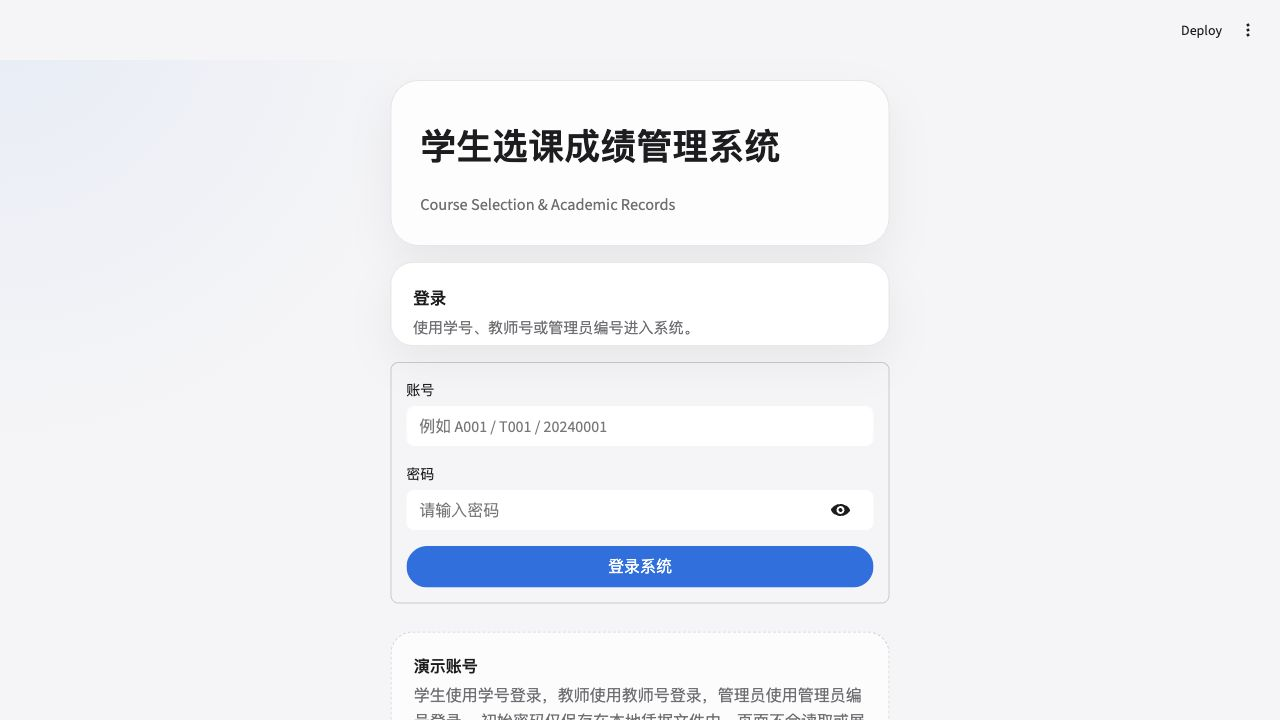
\includegraphics[width=0.95\textwidth]{ui/01_login.png}
    \caption{系统登录界面}
    \label{fig:ui-login}
\end{figure}

图 \ref{fig:ui-student-dashboard} 展示学生端首页。该页面汇总已选课程、本学期课程、已完成课程和绩点等信息，底层数据来自 \code{enrollment}、课程教学表以及绩点统计视图。

\begin{figure}[htbp]
    \centering
    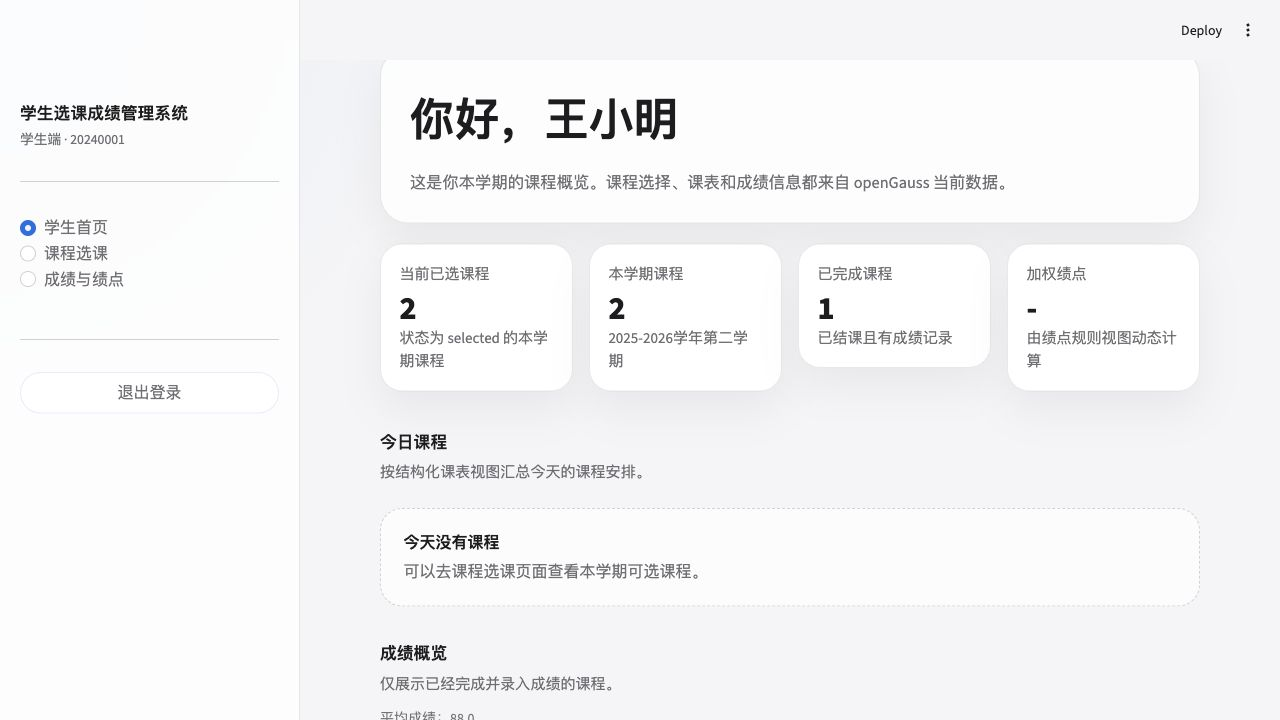
\includegraphics[width=0.95\textwidth]{ui/02_student_dashboard.png}
    \caption{学生端课程概览界面}
    \label{fig:ui-student-dashboard}
\end{figure}

图 \ref{fig:ui-teacher-dashboard} 展示教师端首页。教师端重点呈现本人负责的教学班、学生人数、待录入成绩和成绩录入进度，体现了 \code{teacher}、\code{course_offering}、\code{enrollment} 与成绩服务之间的关系。

\begin{figure}[htbp]
    \centering
    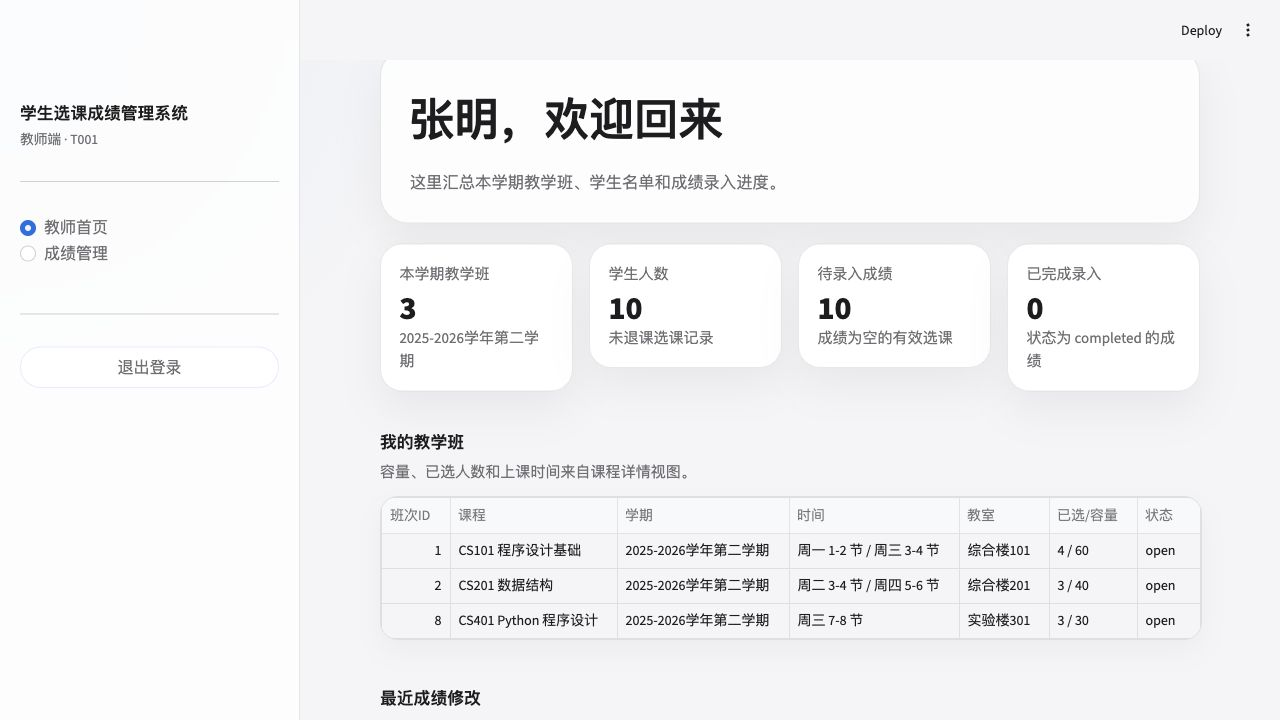
\includegraphics[width=0.95\textwidth]{ui/06_teacher_dashboard.png}
    \caption{教师端教学任务概览界面}
    \label{fig:ui-teacher-dashboard}
\end{figure}

图 \ref{fig:ui-admin-dashboard} 展示管理员端首页。管理员端聚合学生、教师、课程、教学班、当前选课和成绩日志数量，主要用于运行维护和数据质量观察。

\begin{figure}[htbp]
    \centering
    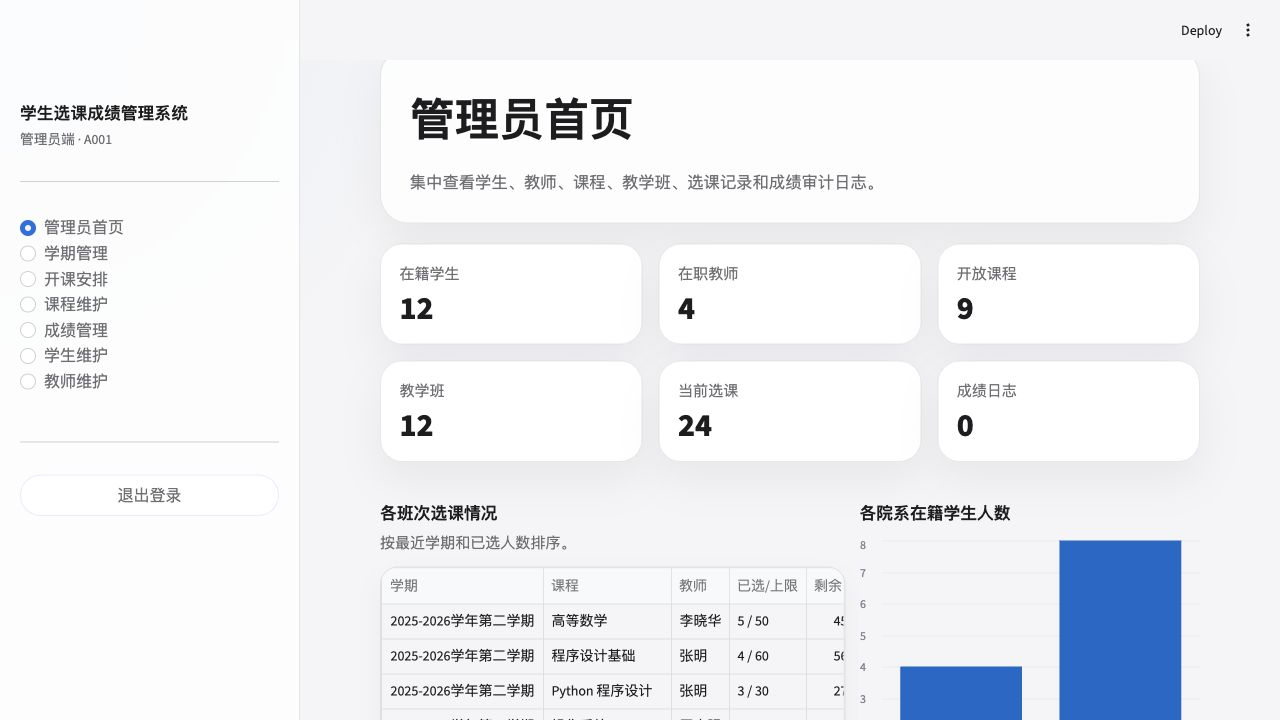
\includegraphics[width=0.95\textwidth]{ui/08_admin_dashboard.png}
    \caption{管理员端系统概览界面}
    \label{fig:ui-admin-dashboard}
\end{figure}

课程查询、学生课表、成绩录入和成绩审计日志等细分页面在演示环境中可继续截图补充。截图索引文件 \code{report/UI_SCREENSHOT_INDEX.md} 记录了各页面截图与报告位置的对应关系；尚未插入 PDF 的页面列入 \code{report/UI_SCREENSHOT_TODO.md}，避免引用不存在的图片导致编译失败。

\section{数据安全}

项目中密码以 SHA-256 哈希保存，持久登录 token 以哈希形式存入 \code{user_session}。这比明文保存更安全，但仍可继续改进，例如使用带盐的密码哈希算法、限制登录尝试次数、设置 HTTPS、定期清理过期会话。

\section{后续扩展}

后续可扩展方向包括：行政班实体拆分、生产环境密钥管理、备份恢复脚本、运行监控、更大规模并发压测和报表优化。这些内容可以作为运行维护阶段的设计完善点。

课程结束后的教师评价模块适合作为后续扩展，而不作为本文主线功能。可设计 \code{teaching_evaluation(evaluation_id, enrollment_id, rating, comment, submitted_at)}，其中 \code{UNIQUE(enrollment_id)} 保证一次选课最多评价一次，\code{CHECK(rating BETWEEN 1 AND 5)} 保证评分合法，触发器可检查只有 \code{completed} 的选课记录且教学班结束后才能评价。教师端只查看 \code{v_teacher_evaluation_summary} 等聚合视图，避免直接暴露学生身份；管理员可根据管理需要查看明细或审计数据。

\chapter{总结与不足}

\section{系统设计总结}

本项目围绕高校选课业务建立了较完整的关系数据库模型。系统区分课程定义和开课班次，使用 \code{enrollment} 转换学生与教学班之间的多对多联系，使用 \code{course_schedule} 结构化表达上课时间片，并通过 \code{course_prerequisite} 表示课程先修自关联。当前数据库结构由 \code{opengauss_setup/sql/init.sql} 和后续迁移脚本维护，共包含 15 张主要表。

\section{课程知识点体现}

项目较好体现了数据库原理2的多个重点内容：

\begin{enumerate}
  \item 数据库设计流程：报告按规划、需求、概念、逻辑、规范化、物理和运行维护展开。
  \item ER 建模：实体、属性、联系和基数均能从真实表结构中抽取。
  \item 关系模型：M:N 联系通过 \code{enrollment} 和 \code{course_prerequisite} 转换为关系模式。
  \item 规范化：通过删除 \code{schedule_text}、\code{selected_count}、\code{gpa_point} 等风险字段，核心表更接近 3NF。
  \item 完整性：主键、外键、唯一约束、CHECK、DEFAULT 和触发器共同维护数据正确性。
  \item 事务与锁：选课流程使用 \code{select_course_tx()}、\code{DBSession} 和 \code{SELECT ... FOR UPDATE} 控制并发。
  \item 物理设计：项目为会话、教学班、时间片、选课记录和成绩日志建立了常用索引，并用视图提升查询便利性。
  \item 测试验证：\code{test_triggers_constraints.sql} 覆盖容量、时间冲突、重复选课、先修关系、成绩审计和视图查询等数据库规则。
\end{enumerate}

\section{项目不足}

当前不足主要包括：同课跨班重复选择限制尚未完全固化；数据库级权限、备份恢复、运行监控和多连接并发压测还不完善；当前使用普通视图而非物化视图，统计报表在数据量很大时仍需进一步评估性能。

\section{后续改进}

如果继续完善项目，优先级较高的数据库相关功能包括：

\begin{enumerate}
  \item 为同课跨班重复选择设计跨表触发器或培养方案规则表。
  \item 增加多连接并发压测，验证最后一个名额抢课时的锁等待和回滚行为。
  \item 建立更完整的数据库管理方案，包括数据库级角色权限、备份恢复和迁移版本管理。
\end{enumerate}

总体而言，本项目已经不是简单的页面 CRUD 程序，而是能够体现数据库设计流程、范式理论、完整性约束、事务锁机制和运行维护思路的数据库应用系统。报告中的不足部分也说明数据库设计需要随着业务规则和运行环境持续迭代。

\clearpage
\appendix
\chapter{关键 SQL 与测试摘录}

\section{选课事务函数摘录}

本系统通过 \code{select_course_tx()} 封装数据库层选课入口。函数在调用方事务中执行，先锁定同一学生同一教学班的既有选课记录，再锁定目标教学班，最终由 \code{trg_enrollment_guard} 完成完整性兜底。

\begin{lstlisting}[style=sqlstyle]
CREATE OR REPLACE FUNCTION select_course_tx(
    p_student_id VARCHAR,
    p_offering_id BIGINT
) RETURNS BIGINT AS $$
...
    PERFORM 1
    FROM course_offering
    WHERE offering_id = p_offering_id
    FOR UPDATE;

    INSERT INTO enrollment (student_id, offering_id, status, select_time)
    VALUES (p_student_id, p_offering_id, 'selected', CURRENT_TIMESTAMP)
    RETURNING enrollment_id INTO v_enrollment_id;
...
$$ LANGUAGE plpgsql;
\end{lstlisting}

\section{角色一致性触发器摘录}

角色档案一致性由通用函数和三个触发器共同实现。下面片段说明普通外键之外，系统还会检查账户角色是否与档案表类型匹配。

\begin{lstlisting}[style=sqlstyle]
CREATE OR REPLACE FUNCTION check_user_role_fn(
    p_user_id BIGINT,
    p_expected_role VARCHAR
) RETURNS void AS $$
...
    IF v_role <> p_expected_role THEN
        RAISE EXCEPTION 'User % role is %, expected %',
            p_user_id, v_role, p_expected_role;
    END IF;
END;
$$ LANGUAGE plpgsql;

CREATE TRIGGER trg_student_role_check
BEFORE INSERT OR UPDATE OF user_id ON student
FOR EACH ROW
EXECUTE PROCEDURE trg_profile_role_check_fn('student');
\end{lstlisting}

\section{选课完整性触发器摘录}

\code{trg_enrollment_guard} 不维护 \code{selected_count}，而是在锁定教学班后统计 \code{enrollment} 中的 \code{selected} 记录数。

\begin{lstlisting}[style=sqlstyle]
SELECT course_id, semester_id, max_capacity, status
  INTO v_course_id, v_semester_id, v_max_capacity, v_offering_status
FROM course_offering
WHERE offering_id = NEW.offering_id
FOR UPDATE;

SELECT COUNT(*) INTO v_selected_count
FROM enrollment e
WHERE e.offering_id = NEW.offering_id
  AND e.status = 'selected'
  AND (v_old_enrollment_id IS NULL OR e.enrollment_id <> v_old_enrollment_id);

IF v_selected_count >= v_max_capacity THEN
    RAISE EXCEPTION 'Course offering % is full', NEW.offering_id;
END IF;
\end{lstlisting}

同课跨班限制也由同一触发器完成。该规则需要同时查询 \code{enrollment} 与 \code{course_offering}，因此不适合只用单表唯一约束表达。

\begin{lstlisting}[style=sqlstyle]
SELECT COUNT(*) INTO v_same_course_count
FROM enrollment e
JOIN course_offering co_same
  ON co_same.offering_id = e.offering_id
WHERE e.student_id = NEW.student_id
  AND e.status = 'selected'
  AND co_same.semester_id = v_semester_id
  AND co_same.course_id = v_course_id
  AND co_same.offering_id <> NEW.offering_id;

IF v_same_course_count > 0 THEN
    RAISE EXCEPTION
        'Student % has already selected another offering for course %',
        NEW.student_id, v_course_id;
END IF;
\end{lstlisting}

\section{成绩审计触发器摘录}

成绩审计触发器要求业务层在同一事务中传入当前操作者，避免把日志操作者写死为管理员或空值。

\begin{lstlisting}[style=sqlstyle]
BEGIN
    v_changed_by_user_id := current_setting('app.current_user_id')::BIGINT;
EXCEPTION WHEN OTHERS THEN
    RAISE EXCEPTION
      'Score update requires app.current_user_id in the current transaction';
END;

INSERT INTO score_change_log
    (enrollment_id, old_score, new_score, changed_by_user_id, reason)
VALUES
    (NEW.enrollment_id, OLD.final_score, NEW.final_score,
     v_changed_by_user_id, v_reason);
\end{lstlisting}

\section{视图 SQL 摘录}

\code{v_offering_selected_count} 通过聚合实时得到已选人数和剩余容量，使基础表无需保存派生字段 \code{selected_count}。

\begin{lstlisting}[style=sqlstyle]
CREATE OR REPLACE VIEW v_offering_selected_count AS
SELECT
    co.offering_id,
    co.max_capacity,
    COALESCE(COUNT(e.enrollment_id), 0)::INTEGER AS selected_count,
    (co.max_capacity - COALESCE(COUNT(e.enrollment_id), 0))::INTEGER
        AS remaining_capacity
FROM course_offering co
LEFT JOIN enrollment e
  ON e.offering_id = co.offering_id
 AND e.status = 'selected'
GROUP BY co.offering_id, co.max_capacity;
\end{lstlisting}

\section{SQL 测试结果摘录}

\code{opengauss_setup/sql/test_triggers_constraints.sql} 使用事务和匿名块捕获预期异常，最后执行 \code{ROLLBACK}，不会污染样例数据。测试覆盖角色错配、先修自指、先修环路、容量超选、时间冲突、同课跨班、重复选课、成绩审计、退课限制和视图查询。一次测试输出摘录如下：

\begin{lstlisting}[style=codestyle]
PASS role check teacher-as-student failed
PASS self prerequisite failed
PASS prerequisite cycle failed
PASS capacity full failed
PASS timetable conflict failed
PASS same course different offering failed
PASS unique student/offering failed
PASS score update without user failed
PASS score audit trigger inserted log row
PASS completed enrollment drop failed
Trigger and constraint tests finished with rollback.
\end{lstlisting}

\section{并发抢课测试脚本摘录}

\code{scripts/concurrency_enrollment_test.py} 用于在两个独立数据库连接中同时调用 \code{select_course_tx()}。并发测试在本地 openGauss 容器中构造容量为 1 的教学班，最终只有一个学生选课成功。测试输出摘录如下：

\begin{lstlisting}[style=codestyle]
TST_CONC_STU_1: FAILED - Course offering 42 is full
TST_CONC_STU_2: SUCCESS - selected
success_count = 1
failed_count = 1
selected_count_in_db = 1
\end{lstlisting}

\section{数据库角色授权脚本摘录}

\code{grant_roles_20260608.sql} 体现数据库管理中的最小权限思想。本地生成的 \code{opengauss_setup/sql/local/grant_demo_db_accounts_20260611.sql} 用于演示数据库登录账号与角色绑定。由于本地绑定脚本包含数据库账号密码，不进入公开仓库和报告正文。

\begin{lstlisting}[style=sqlstyle]
CREATE ROLE db_student_role;
CREATE ROLE db_teacher_role;
CREATE ROLE db_admin_role;
CREATE ROLE db_app_role;

REVOKE ALL ON ALL TABLES IN SCHEMA public FROM PUBLIC;

GRANT SELECT ON
    v_course_offering_detail,
    v_offering_selected_count
TO db_student_role;

GRANT EXECUTE ON FUNCTION select_course_tx(VARCHAR, BIGINT)
TO db_app_role;
\end{lstlisting}

\section{演示账号凭据策略摘录}

演示业务账号使用业务身份编号作为登录名：学生用学号，教师用教师号，管理员用管理员编号。明文初始密码只保存在本地 \code{secrets/DEMO_ACCOUNT_CREDENTIALS.md}，SQL 中只保存 SHA-256 哈希。

\begin{lstlisting}[style=codestyle]
student username = student.student_id      # e.g. 20240001
teacher username = teacher.teacher_id      # e.g. T001
admin username   = admin_profile.admin_id  # e.g. A001

python3 scripts/generate_large_demo_dataset.py
\end{lstlisting}

\section{绩点规则版本化 SQL 摘录}

绩点不作为 \code{enrollment} 的基础字段保存，而是由规则版本和成绩区间计算。下面摘录展示 \code{grade_policy}、\code{grade_scale} 和计算函数的核心结构。

\begin{lstlisting}[style=sqlstyle]
CREATE TABLE grade_policy (
    policy_id BIGSERIAL PRIMARY KEY,
    policy_code VARCHAR(30) NOT NULL,
    policy_name VARCHAR(100) NOT NULL,
    version_no VARCHAR(20) NOT NULL,
    effective_from DATE NOT NULL,
    effective_to DATE,
    status VARCHAR(20) NOT NULL DEFAULT 'active',
    UNIQUE (policy_code, version_no)
);

CREATE TABLE grade_scale (
    scale_id BIGSERIAL PRIMARY KEY,
    policy_id BIGINT NOT NULL REFERENCES grade_policy(policy_id),
    min_score DECIMAL(5,2) NOT NULL,
    max_score DECIMAL(5,2) NOT NULL,
    gpa_point DECIMAL(3,2) NOT NULL,
    grade_label VARCHAR(10)
);
\end{lstlisting}

\begin{lstlisting}[style=sqlstyle]
CREATE OR REPLACE FUNCTION calculate_gpa(
    p_score DECIMAL,
    p_policy_id BIGINT
) RETURNS DECIMAL(3,2) AS $$
...
    SELECT COUNT(*), MIN(gpa_point)
      INTO v_match_count, v_gpa
    FROM grade_scale
    WHERE policy_id = p_policy_id
      AND p_score >= min_score
      AND p_score <= max_score;
...
$$ LANGUAGE plpgsql;
\end{lstlisting}

\code{test_grade_policy.sql} 覆盖绩点规则插入、区间重叠失败、\code{calculate_gpa(95)}、\code{calculate_gpa(59)} 以及绩点视图查询。回滚型测试输出摘录如下：

\begin{lstlisting}[style=codestyle]
PASS calculate_gpa 95 -> 4.00
PASS calculate_gpa 59 -> 0.00
PASS overlap grade scale failed
PASS v_enrollment_grade_detail returned ... GPA rows
PASS v_student_gpa_summary returned ... summary rows
Grade policy tests finished with rollback.
\end{lstlisting}

\section{大规模演示数据验证摘录}

最终演示数据由 \code{scripts/generate_large_demo_dataset.py} 使用固定随机种子生成，导入脚本位于本地 \code{opengauss_setup/sql/local/seed_large_demo_dataset_20260611.sql}。明文初始密码只保存在本地 \code{secrets/DEMO_ACCOUNT_CREDENTIALS.md}，不进入报告正文。数据规模摘要如下：

\begin{lstlisting}[style=codestyle]
Departments: 4
Students: 100
Teachers: 30
Courses: 50
Course offerings: 175
Schedule slots: 214
Enrollments: 1480
Completed enrollments: 1000
Selected enrollments: 425
Dropped enrollments: 55
Score change logs: 80
\end{lstlisting}

\code{validate_large_demo_dataset.sql} 对大规模数据进行只读验证，检查教学班容量、教室容量、重复选课、同课跨班、时间冲突、先修课、成绩状态、账号角色、先修环路和成绩审计日志。关键检查片段如下：

\begin{lstlisting}[style=sqlstyle]
WITH selected_count AS (
    SELECT offering_id, COUNT(*) AS selected_count
    FROM enrollment
    WHERE status = 'selected'
    GROUP BY offering_id
)
SELECT COUNT(*) AS violation_count
FROM course_offering co
LEFT JOIN selected_count sc ON sc.offering_id = co.offering_id
WHERE COALESCE(sc.selected_count, 0) > co.max_capacity;

SELECT COUNT(*) AS violation_count
FROM enrollment e1
JOIN enrollment e2
  ON e1.student_id = e2.student_id
 AND e1.enrollment_id < e2.enrollment_id
JOIN course_offering co1 ON co1.offering_id = e1.offering_id
JOIN course_offering co2 ON co2.offering_id = e2.offering_id
JOIN course_schedule cs1 ON cs1.offering_id = co1.offering_id
JOIN course_schedule cs2 ON cs2.offering_id = co2.offering_id
WHERE e1.status = 'selected'
  AND e2.status = 'selected'
  AND co1.semester_id = co2.semester_id
  AND cs1.weekday = cs2.weekday
  AND cs1.start_section <= cs2.end_section
  AND cs1.end_section >= cs2.start_section;
\end{lstlisting}

本地 openGauss 验证结果显示，容量超限、教室容量超限、重复选课、同课跨班、时间冲突、先修课不满足、成绩状态异常、角色错配、先修自指或环路、审计日志无效引用等违规项均为 0。绩点视图 smoke check 返回 \code{v_enrollment_grade_detail} 1480 行、\code{v_student_gpa_summary} 284 行。

\section{教师评价扩展设计}

教师评价不作为本系统当前主线功能实现。若后续扩展，可新增 \code{teaching_evaluation} 表，并把它作为选课记录完成后的附属业务实体。

\begin{lstlisting}[style=sqlstyle]
teaching_evaluation(
    evaluation_id,
    enrollment_id,
    rating,
    comment,
    submitted_at
)
\end{lstlisting}

设计上应保证一个 \code{enrollment} 最多评价一次，评分范围为 1 到 5，且只有 \code{completed} 状态的选课记录可以评价。教师侧宜查看聚合结果，例如平均分与评价人数，而不是直接查看学生身份。


\chapter*{参考资料}
\addcontentsline{toc}{chapter}{参考资料}
\begin{enumerate}
  \item 项目仓库文件：\code{opengauss_setup/sql/init.sql}、\code{services/*.py}、\code{db/connection.py}、\code{README.md}。
  \item 数据库原理2课堂笔记：数据库设计流程、范式、事务、并发控制、完整性、安全性相关章节。
  \item openGauss 与 PostgreSQL 兼容 SQL 特性文档，用于理解主键、外键、CHECK、索引和 \code{SELECT ... FOR UPDATE}。
\end{enumerate}

\end{document}
